\documentclass[conference]{IEEEtran}
\usepackage[utf8]{inputenc}
\usepackage[T1]{fontenc}
\usepackage{amsmath,amssymb}
\usepackage{graphicx}
\usepackage{booktabs}
\usepackage{multirow}
\usepackage[hidelinks]{hyperref}
\graphicspath{{figures/}}

\newcommand{\Fmax}{\bar{F}}
% generated by experiments/make_numbers.py -- do not edit
\newcommand{\agilityFastRate}{3/6}
\newcommand{\agilityFastV}{0.25}
\newcommand{\agilityRate}{10/10}
\newcommand{\agilityV}{0.23}
\newcommand{\allMotorMass}{48.6}
\newcommand{\authGaitAll}{0.00}
\newcommand{\authGaitBom}{0.00}
\newcommand{\authGaitHip}{0.87}
\newcommand{\authGaitKnee}{0.61}
\newcommand{\authHomeAll}{1.01}
\newcommand{\authHomeBom}{0.66}
\newcommand{\authShortGaitAll}{10}
\newcommand{\authShortGaitBom}{13}
\newcommand{\authShortHomeAll}{0}
\newcommand{\authShortHomeBom}{6}
\newcommand{\bearingMass}{1.89}
\newcommand{\bearingPerDof}{70}
\newcommand{\benchAnkleArmA}{55}
\newcommand{\benchAnkleArmB}{66}
\newcommand{\benchAnkleMoment}{16}
\newcommand{\benchLegSink}{12}
\newcommand{\benchLegT}{41}
\newcommand{\benchLegTTwo}{55}
\newcommand{\benchWaistSink}{24}
\newcommand{\bomMass}{16.1}
\newcommand{\bomMassFixed}{19.4}
\newcommand{\carryHinEight}{6.0}
\newcommand{\carryHinSixteen}{8.0}
\newcommand{\carryHinSlope}{16}
\newcommand{\carryHinTwelve}{6.0}
\newcommand{\carryHybEight}{1.5}
\newcommand{\carryHybSixteen}{3.0}
\newcommand{\carryHybSlope}{53}
\newcommand{\carryHybTwelve}{2.0}
\newcommand{\cellChainDroop}{29}
\newcommand{\cellChainMax}{5}
\newcommand{\cellChainPer}{5.9}
\newcommand{\cgCables}{306}
\newcommand{\cgCellStruts}{39}
\newcommand{\cgClusterStruts}{27}
\newcommand{\cgDof}{210}
\newcommand{\cgLoadFail}{5}
\newcommand{\cgNodeLoad}{637}
\newcommand{\cgNodeMargin}{3.7}
\newcommand{\cgPreNeeded}{1000}
\newcommand{\cgPreSettle}{48}
\newcommand{\cgSettle}{6}
\newcommand{\cgStruts}{66}
\newcommand{\cpayAllCiHi}{83}
\newcommand{\cpayAllCiLo}{65}
\newcommand{\cpayAllPct}{75}
\newcommand{\cpayAllRate}{60/80}
\newcommand{\cpayEightCiHi}{89}
\newcommand{\cpayEightCiLo}{40}
\newcommand{\cpayEightRate}{7/10}
\newcommand{\cpayEightV}{0.19}
\newcommand{\cpayFourCiHi}{83}
\newcommand{\cpayFourCiLo}{31}
\newcommand{\cpayFourRate}{6/10}
\newcommand{\cpayFourV}{0.19}
\newcommand{\cpaySixCiHi}{89}
\newcommand{\cpaySixCiLo}{40}
\newcommand{\cpaySixRate}{7/10}
\newcommand{\cpaySixV}{0.20}
\newcommand{\cpaySixteenCiHi}{98}
\newcommand{\cpaySixteenCiLo}{60}
\newcommand{\cpaySixteenRate}{9/10}
\newcommand{\cpaySixteenV}{0.17}
\newcommand{\cpayTenCiHi}{83}
\newcommand{\cpayTenCiLo}{31}
\newcommand{\cpayTenRate}{6/10}
\newcommand{\cpayTenV}{0.20}
\newcommand{\cpayTwelveCiHi}{89}
\newcommand{\cpayTwelveCiLo}{40}
\newcommand{\cpayTwelveRate}{7/10}
\newcommand{\cpayTwelveV}{0.19}
\newcommand{\cpayTwentyCiHi}{98}
\newcommand{\cpayTwentyCiLo}{60}
\newcommand{\cpayTwentyRate}{9/10}
\newcommand{\cpayTwentyV}{0.17}
\newcommand{\cpayTwoCiHi}{98}
\newcommand{\cpayTwoCiLo}{60}
\newcommand{\cpayTwoRate}{9/10}
\newcommand{\cpayTwoV}{0.20}
\newcommand{\distalN}{10}
\newcommand{\distalOk}{6}
\newcommand{\distalRate}{6/10}
\newcommand{\distalSpeed}{0.17}
\newcommand{\eOneBWRigidCrash}{14}
\newcommand{\eOneBWRigidStumble}{5}
\newcommand{\eOneBWTsgCrash}{36}
\newcommand{\eOneBWTsgStumble}{5}
\newcommand{\eOneCrossover}{0.2}
\newcommand{\eOneDeltaHeldCrash}{+3}
\newcommand{\eOneDeltaHeldStumble}{+2}
\newcommand{\eOneDeltaPassiveCrash}{+154}
\newcommand{\eOneDeltaPassiveStumble}{+14}
\newcommand{\eOneHeldRigidCrash}{4133}
\newcommand{\eOneHeldRigidStumble}{1820}
\newcommand{\eOneHeldTsgCrash}{4262}
\newcommand{\eOneHeldTsgStumble}{1853}
\newcommand{\eOneMismatched}{20}
\newcommand{\eOnePassiveFell}{7}
\newcommand{\eOnePassiveN}{7}
\newcommand{\eOnePassiveRigidCrash}{3785}
\newcommand{\eOnePassiveRigidStumble}{1273}
\newcommand{\eOnePassiveTsgCrash}{9629}
\newcommand{\eOnePassiveTsgStumble}{1454}
\newcommand{\eSixSummary}{Capping every joint at the torque the full cable network can deliver over the gait leaves the planner 7/10 successful walks at 0.17\,m/s; capping at the worst-case bound gives 3/6; and capping at what the 36-motor bill of materials can deliver gives 0/10. A gait therefore exists inside the envelope of the full network but not inside the envelope of the actuation set we specified: the shortfall is in the bill of materials, not in the topology.}
\newcommand{\eSixtendonallRate}{7/10}
\newcommand{\eSixtendonbomRate}{0/10}
\newcommand{\eSixtendonminRate}{3/6}
\newcommand{\eThreeAdvEight}{0/4}
\newcommand{\eThreeAdvFour}{4/4}
\newcommand{\eThreeAdvTwo}{4/4}
\newcommand{\eThreeBaseMargin}{1.01}
\newcommand{\eThreeBelowOne}{44}
\newcommand{\eThreeLegEight}{8/8}
\newcommand{\eThreeLegFour}{8/8}
\newcommand{\eThreeLegTwo}{8/8}
\newcommand{\eThreeRandEight}{8/8}
\newcommand{\eThreeRandFour}{8/8}
\newcommand{\eThreeRandTwo}{8/8}
\newcommand{\eThreeSinglesN}{15}
\newcommand{\eThreeSinglesOk}{15}
\newcommand{\extraMotorMass}{3.2}
\newcommand{\freeZend}{-0.03}
\newcommand{\freeZstart}{0.94}
\newcommand{\gaitClr}{42}
\newcommand{\hingeConstrainedDof}{57}
\newcommand{\hingeDof}{27}
\newcommand{\hingeDofCount}{27}
\newcommand{\hingeSegments}{14}
\newcommand{\hsCarryMax}{2.0}
\newcommand{\hsCarryUtil}{65}
\newcommand{\hsCarryWaistT}{88}
\newcommand{\hsPayEightRate}{3/10}
\newcommand{\hsPayEightV}{0.20}
\newcommand{\hsPayFiveRate}{9/10}
\newcommand{\hsPayFiveV}{0.18}
\newcommand{\hsPayTwelveRate}{0/10}
\newcommand{\hsPayTwelveV}{0.00}
\newcommand{\hsPayTwoRate}{10/10}
\newcommand{\hsPayTwoV}{0.18}
\newcommand{\hsSpdFortyFiveRate}{6/6}
\newcommand{\hsSpdFortyFiveV}{0.19}
\newcommand{\hsSpdSixtyRate}{0/6}
\newcommand{\hsSpdSixtyV}{0.00}
\newcommand{\hsSpdThirtyRate}{6/6}
\newcommand{\hsSpdThirtyV}{0.10}
\newcommand{\hybridAnkleDuty}{7}
\newcommand{\hybridAnklePeak}{250}
\newcommand{\hybridHipHw}{257}
\newcommand{\hybridJointDuty}{9}
\newcommand{\hybridJointHw}{0.8}
\newcommand{\hybridKneeHw}{142}
\newcommand{\hybridMass}{20.1}
\newcommand{\hybridRate}{10/10}
\newcommand{\hybridSpeed}{0.18}
\newcommand{\jcRAnkleRate}{5/5}
\newcommand{\jcRAnkleV}{0.21}
\newcommand{\jcRBothRate}{5/5}
\newcommand{\jcRBothV}{0.23}
\newcommand{\jcRWaistRate}{0/5}
\newcommand{\jcRWaistTunedRate}{4/5}
\newcommand{\jcRWaistTunedTorso}{1.28}
\newcommand{\jcRWaistTunedV}{0.18}
\newcommand{\jcRWaistV}{0.00}
\newcommand{\jointGeomElasticRope}{0.2}
\newcommand{\jointGeomElasticSoft}{67}
\newcommand{\jointImpactCableFive}{209}
\newcommand{\jointImpactCableTen}{282}
\newcommand{\jointImpactCableTwenty}{388}
\newcommand{\jointImpactDeltaFive}{27}
\newcommand{\jointImpactDeltaTen}{30}
\newcommand{\jointImpactDeltaTwenty}{32}
\newcommand{\jointImpactHi}{32}
\newcommand{\jointImpactLo}{27}
\newcommand{\jointImpactPinFive}{287}
\newcommand{\jointImpactPinTen}{404}
\newcommand{\jointImpactPinTwenty}{568}
\newcommand{\jointOverlapFrac}{0.2}
\newcommand{\jointOverlapMm}{60}
\newcommand{\jointPreRatioRope}{1.06}
\newcommand{\jointPreRatioSeries}{1.33}
\newcommand{\jointPreRatioSoft}{23.22}
\newcommand{\kModelMax}{2500}
\newcommand{\kModelMin}{600}
\newcommand{\kRopeMax}{7.1}
\newcommand{\kRopeMin}{0.3}
\newcommand{\kSeriesMax}{168}
\newcommand{\kSeriesMin}{20}
\newcommand{\lbCables}{135}
\newcommand{\lbDroop}{18}
\newcommand{\lbStruts}{18}
\newcommand{\membersMass}{5.64}
\newcommand{\nodeCount}{93}
\newcommand{\nodeMass}{0.84}
\newcommand{\numActuatable}{114}
\newcommand{\numCableEnds}{444}
\newcommand{\numDof}{27}
\newcommand{\numDrivenCables}{72}
\newcommand{\numEndpoints}{372}
\newcommand{\numMotors}{36}
\newcommand{\numMotorsFixed}{43}
\newcommand{\numPassiveCables}{42}
\newcommand{\numStruts}{60}
\newcommand{\numTendonCable}{222}
\newcommand{\numTendonTorque}{186}
\newcommand{\payTenRate}{10/10}
\newcommand{\payTenV}{0.19}
\newcommand{\physOneHeldFifty}{+73}
\newcommand{\physOneHeldFive}{-25}
\newcommand{\physOneHeldHundred}{+96}
\newcommand{\physOneHeldTen}{+1}
\newcommand{\physOneHeldThirty}{+53}
\newcommand{\physOneHeldTwenty}{+41}
\newcommand{\physOneLimpFifty}{+177}
\newcommand{\physOneLimpFive}{+112}
\newcommand{\physOneLimpHundred}{+197}
\newcommand{\physOneLimpTen}{+110}
\newcommand{\physOneLimpThirty}{+142}
\newcommand{\physOneLimpTwenty}{+113}
\newcommand{\physTwoCableRatio}{18}
\newcommand{\physTwoEngaged}{-2}
\newcommand{\physTwoHigh}{591}
\newcommand{\physTwoNoCables}{13}
\newcommand{\physTwoNominal}{615}
\newcommand{\physTwoZeroPre}{226}
\newcommand{\rHaveHip}{37.5}
\newcommand{\rHaveKnee}{47.6}
\newcommand{\rNeedHip}{53.3}
\newcommand{\realtimeFactor}{0.60}
\newcommand{\realtimeN}{142}
\newcommand{\ropeBLLeg}{12.8}
\newcommand{\ropeDMax}{4.0}
\newcommand{\ropeDMin}{1.0}
\newcommand{\ropeMass}{0.10}
\newcommand{\ropeUtilRms}{12}
\newcommand{\rpayEightRate}{5/6}
\newcommand{\rpayFourRate}{6/6}
\newcommand{\rpaySixRate}{5/6}
\newcommand{\rpaySixteenRate}{3/6}
\newcommand{\rpayTenRate}{3/6}
\newcommand{\rpayTwelveRate}{6/6}
\newcommand{\rpayTwentyRate}{4/6}
\newcommand{\rpayTwoRate}{3/6}
\newcommand{\shellAllowance}{0.26}
\newcommand{\singleLoopHip}{56}
\newcommand{\singleLoopKnee}{71}
\newcommand{\spdFortyFiveN}{10}
\newcommand{\spdFortyFiveOk}{1}
\newcommand{\spdFortyFiveRate}{1/10}
\newcommand{\spdFortyFiveV}{0.29}
\newcommand{\spdFortyN}{10}
\newcommand{\spdFortyOk}{3}
\newcommand{\spdFortyRate}{3/10}
\newcommand{\spdFortyV}{0.26}
\newcommand{\spdTenN}{10}
\newcommand{\spdTenOk}{0}
\newcommand{\spdTenRate}{0/10}
\newcommand{\spdTenV}{---}
\newcommand{\spdThirtyFiveN}{10}
\newcommand{\spdThirtyFiveOk}{6}
\newcommand{\spdThirtyFiveRate}{6/10}
\newcommand{\spdThirtyFiveV}{0.24}
\newcommand{\spdThirtyRate}{7/10}
\newcommand{\spdThirtyV}{0.21}
\newcommand{\spdTwentyN}{10}
\newcommand{\spdTwentyOk}{8}
\newcommand{\spdTwentyRate}{8/10}
\newcommand{\spdTwentyV}{0.13}
\newcommand{\stiffCablesRatio}{2.4}
\newcommand{\stiffCoHi}{115}
\newcommand{\stiffCoKnee}{96}
\newcommand{\stiffCoLo}{14}
\newcommand{\stiffCoRatio}{8.4}
\newcommand{\stiffGapRope}{1685}
\newcommand{\stiffGapSeries}{46}
\newcommand{\stiffLinearity}{0.5}
\newcommand{\stiffNoCables}{5.4}
\newcommand{\stiffNominal}{12.6}
\newcommand{\stiffPreHi}{16.6}
\newcommand{\stiffPreLo}{11.6}
\newcommand{\stiffPreRatio}{1.4}
\newcommand{\stiffProbe}{200}
\newcommand{\stiffSensTenHi}{+21}
\newcommand{\stiffSensTenLo}{+5}
\newcommand{\stiffZeroPre}{13.3}
\newcommand{\strutFittingMass}{0.36}
\newcommand{\strutLenMax}{589}
\newcommand{\strutLenMin}{32}
\newcommand{\strutLoadDrop}{3210}
\newcommand{\strutLoadStand}{90}
\newcommand{\strutLoadStumble}{485}
\newcommand{\strutMarginDrop}{0.7}
\newcommand{\strutMarginStand}{26.1}
\newcommand{\strutMarginStumble}{4.9}
\newcommand{\strutMassSized}{0.54}
\newcommand{\strutOdMax}{20}
\newcommand{\strutOdMin}{12}
\newcommand{\strutPeakN}{51}
\newcommand{\strutSpecMass}{1.03}
\newcommand{\strutTubeMass}{0.67}
\newcommand{\strutWall}{0.5}
\newcommand{\strutWeakestPcr}{2358}
\newcommand{\strutWorstMargin}{6.0}
\newcommand{\takeupMax}{202}
\newcommand{\takeupMin}{66}
\newcommand{\tendonSpecMass}{1.88}
\newcommand{\tensBusiestRms}{1020}
\newcommand{\tensNeedEight}{2557}
\newcommand{\tensNeedFour}{3310}
\newcommand{\tensNeedSixteen}{2782}
\newcommand{\tensNeedTwelve}{2559}
\newcommand{\tensNeedTwenty}{2619}
\newcommand{\tensNeeded}{2407}
\newcommand{\tensPeak}{1500}
\newcommand{\tensResid}{24}
\newcommand{\tensResidEight}{30}
\newcommand{\tensResidFour}{30}
\newcommand{\tensResidSixteen}{30}
\newcommand{\tensResidTwelve}{39}
\newcommand{\tensResidTwenty}{31}
\newcommand{\tensSatEight}{41}
\newcommand{\tensSatFour}{42}
\newcommand{\tensSatPct}{10.9}
\newcommand{\tensSatSixteen}{46}
\newcommand{\tensSatTwelve}{48}
\newcommand{\tensSatTwenty}{75}
\newcommand{\termMass}{1.78}
\newcommand{\walkCiHi}{89}
\newcommand{\walkCiLo}{40}
\newcommand{\walkCot}{3.3}
\newcommand{\walkN}{10}
\newcommand{\walkOk}{7}
\newcommand{\walkRate}{7/10}
\newcommand{\walkSpeed}{0.21}
\newcommand{\walkSpeedSd}{0.01}
\newcommand{\wcSix}{0}
\newcommand{\wcThree}{0}
\newcommand{\wcTotal}{14}


\title{MPC-based Co-Design of a Tensegrity-based\\27\,DoF Humanoid Robot}

\author{\IEEEauthorblockN{Nikolaus Correll}
\IEEEauthorblockA{Department of Aerospace and Mechanical Engineering\\
University of Notre Dame\\
ncorrell@nd.edu}}

\begin{document}
\maketitle

\begin{abstract}
How much of a humanoid should be joints, and how much can be tensegrity? We
answer by building along the whole axis. At one end, a full-size machine made
only of prestressed cable-and-strut cells stands but cannot be controlled: a
wrench-closure analysis shows why, and a counter-wound cable topology we
derive is necessary before any hinge-free joint can even carry load. At the
other end, a fully hinged 27-DoF variant walks, but pays 1.89\,kg of
bearings, transmits impacts unattenuated, and loses every property prestress
promises. The design this paper argues for is the measured optimum between
them: a 1.68\,m, \hybridMass\,kg hybrid whose hips and knees are bearings
(three-axis gimbals and clevis pins, sized at SF\,2.3 from the measured
1.5\,kN stumble reaction) and whose ankles and waist are genuine tensegrity
joints --- the feet and torso are free bodies held only by cable interfaces
--- with 7-DoF arms whose non-swing joints hold position on servo stiffness.
Under a receding-horizon iLQG controller tracking an analytic gait reference,
the hybrid walks at \hybridSpeed\,m/s in \hybridRate{} of trials, with
\hybridJointHw\,kg of articulation hardware. A joint-count study over
variants of the same machine locates the boundary: rigidizing the tensegrity
joints makes the gait faster but was not more reliable under a fixed
controller, while removing the remaining bearings leaves no controllable
machine at all. Joints buy pose-independent torque and a small planning
abstraction; tensegrity buys impact attenuation ($-27$ to $-32\%$ at the
joint), an order-of-magnitude lighter actuation at compliance-critical
joints, and graceful degradation. The rule the data support: bearings where
the gait's torque lives, cables where the world's impacts arrive.
\end{abstract}

\begin{figure*}[t]
\centering
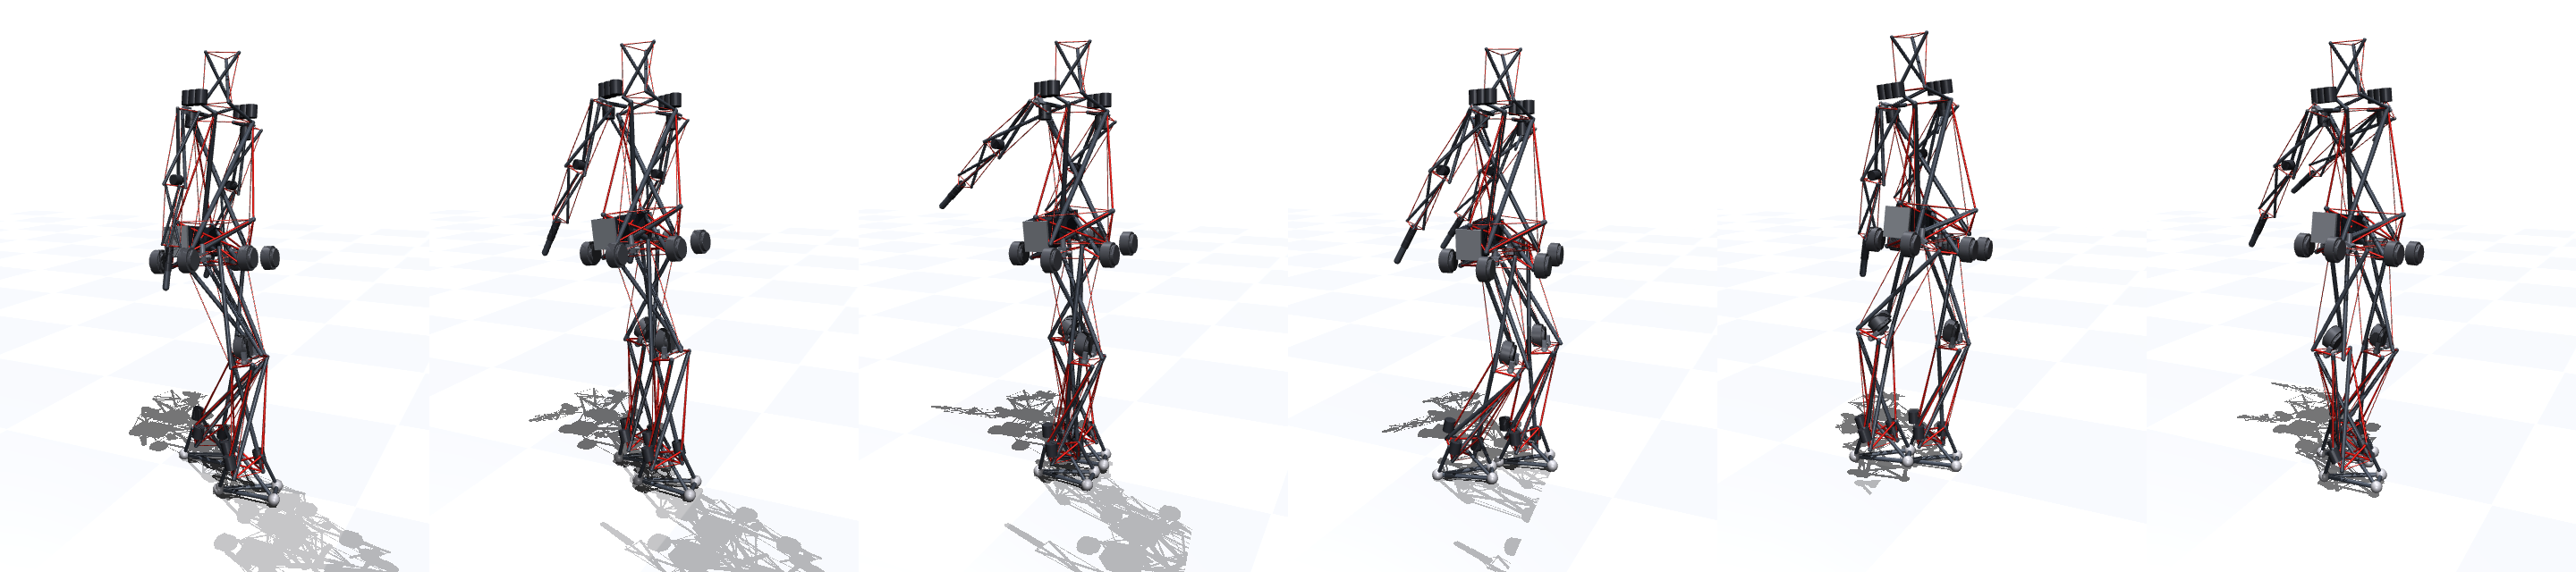
\includegraphics[width=0.99\textwidth]{hybrid_strip.png}
\caption{The hybrid humanoid walking under iLQG (\hybridSpeed\,m/s,
\hybridRate{} of trials). Hips and knees are bearings with proximally mounted
drives; the ankles and waist are tensegrity joints --- the feet and torso are
free bodies held only by counter-wound cable interfaces; the arms are 7\,DoF
with servo-held wrists and shoulders. 1.68\,m, \hybridMass\,kg including two
swappable battery packs.}
\label{fig:sequence}
\end{figure*}

\section{Introduction}
Mass is the binding constraint on humanoid robots. It sets the actuator
torques, which set the motor mass, which sets the battery mass, which sets the
mass again; it sets the energy of every unintended collision; and it is why
machines of human size are dangerous to stand next to. Conventional humanoids
are chains of rigid links with actuators at the joints, an architecture that
concentrates mass distally, makes collisions stiff, and couples structural
strength to structural weight.

Tensegrity structures \cite{fuller1962patent,snelson1965patent} invert this
logic: disconnected struts float in a network of pre-tensioned cables, every
member is loaded along its axis, and the structure's stiffness is a function
of prestress rather than of section. These properties have made tensegrity
attractive for planetary landers and mobile robots
\cite{sabelhaus2015superball,caluwaerts2014design,paul2006locomotion,shah2022tensegrity},
but they have not been carried to a walking machine of human size, and
whether they survive that transition is not something statics can answer.

This paper reports one full iteration of a design loop that uses
model-predictive control as its inner step: we generate a parametric
tensegrity kinematics, test its controllability under tension-only actuation,
size its actuators and members from simulated load traces, and ask a
receding-horizon iLQG controller \cite{li2004ilqr,tassa2012synthesis,
howell2022mjpc} to balance and walk it. Every design change is then justified
by whether it improves the gait.

\textbf{What we find.} The results are stated here and supported in the
sections indicated.
\begin{enumerate}
  \item \emph{The mass payoff is real and is the headline.} At 1.68\,m the
    hybrid masses \hybridMass\,kg where size-matched humanoids mass
    30--80\,kg (Table~\ref{tab:compare}). Compression members are nowhere
    near buckling-critical --- minimum manufacturable wall with
    $\strutWorstMargin\times$ margin (Sec.~\ref{sec:members}) --- and
    articulation hardware is \hybridJointHw\,kg because only eight DoF carry
    bearings.
  \item \emph{Because the structure is the transmission, proximal actuation
    is free, and it is worth something measurable.} Moving the same motor
    masses to the joints they drive costs walk success and speed
    (Sec.~\ref{sec:evidence}).
  \item \emph{Impact tolerance is available to the architecture but not to a
    hinged implementation of it.} With actuation held constant the tension
    network raises peak ground reaction at every drop height
    (Sec.~\ref{sec:evidence}); rebuilt hinge-free with overlapped cages it
    lowers it by \jointImpactLo--\jointImpactHi\%
    (Sec.~\ref{sec:jointimpact}).
  \item \emph{Stiffness is an actuation variable, not an assembly parameter,
    and this is a materials condition rather than a topology one.} Prestress
    tunes stiffness only when the geometric term is comparable to the elastic
    term; with rope it is \jointGeomElasticRope\% of it, hinged or not
    (Sec.~\ref{sec:prestressscaling}). Co-contraction moves stiffness by
    $\stiffCoRatio\times$.
  \item \emph{The binding constraint on cable joints is pose-dependent
    torque authority} (\authShortGaitBom{} of 27 DoFs short mid-stride on the
    fully hinged variant's cable network, Sec.~\ref{sec:authority}) --- which
    is precisely why the hybrid keeps bearings at hips and knees, and the
    joint-count study of Sec.~\ref{sec:jointcount} makes the allocation rule
    quantitative: bearings where the gait's torque lives, cables where
    impacts arrive.
\end{enumerate}

\textbf{Contributions.} (i) A 27-DoF, 1.65\,m tensegrity-based humanoid whose
every segment is a Snelson 3-strut prism cell at the form-found equilibrium
twist, specified down to tube and rope (Sec.~\ref{sec:design}); (ii) a
faithful MuJoCo implementation of tensegrity mechanics with a verification
pipeline whose cable-authority analysis caught three routing errors that would
have left joints uncontrollable (Sec.~\ref{sec:model}); (iii) an MPC
architecture in which iLQG tracks an analytic walking reference, yielding
repeatable straight-line walking where cost-shaping produced only stepping in
place (Sec.~\ref{sec:mpc}); (iv) a simulation-driven dimensioning methodology
that converts gait traces into torque, tension, bandwidth and stroke
requirements and into a bill of materials (Sec.~\ref{sec:codesign}); and (v) a
matched-condition evaluation of the tensegrity case itself
(Sec.~\ref{sec:evidence}), including a configuration- and actuation-aware
authority bound that predicts, and a re-planning experiment that confirms,
where the design falls short.

\section{Related Work and Size-Matched Comparison}
\label{sec:related}

\textbf{Tensegrity robotics.} Following the artistic and architectural origins
of tensegrity \cite{fuller1962patent,snelson1965patent} and its structural
analysis \cite{calladine1978tensegrity,skelton2009tensegrity}, robotic
tensegrities have been demonstrated primarily as rolling or crawling machines:
actuated icosahedra such as NASA's SUPERball
\cite{sabelhaus2015superball,caluwaerts2014design} and earlier strut-cable
crawlers \cite{paul2006locomotion}; the field is surveyed in
\cite{shah2022tensegrity}. Control has been approached by learning
\cite{zhang2017tensegrityrl,surovik2021adaptive} and by optimization, with
model-predictive control and inverse-statics tension distribution demonstrated
on tensegrity spine robots \cite{sabelhaus2018spinempc} --- the closest
precedent for the hierarchical architecture we adopt, though those spines are
few-DoF modules loaded quasi-statically rather than machines that must carry
their own weight through single support. Tensegrity manipulators with
structurally compliant joints \cite{lessard2016manipulator}, modular cells
\cite{zappetti2017modular} and a variable-stiffness spine
\cite{zappetti2020spine} show that limb-like assemblies are feasible;
form-finding is reviewed in \cite{tibert2003form,aloui2019morphogenesis}.

\textbf{Tendon-driven humanoids.} Full-size tendon-driven humanoids are
established: the JSK musculoskeletal line --- Kenshiro
\cite{nakanishi2013kenshiro} and Kengoro \cite{asano2017kengoro} --- routes on
the order of a hundred Dyneema muscles over a human-mimetic skeleton, with
proximal motor placement and the same unilateral tension constraint we face,
as does the ECCE/Anthrob line \cite{wittmeier2013anthropomimetic}. What
distinguishes the present design is not tendon drive but that the tendons
\emph{are} the structure: the prestressed network that applies joint moments
also carries the structural tension, so there is no separate skeleton for the
muscles to act on. Soft exosuits \cite{quinlivan2017exosuit} established that
textile load paths carry forces of this magnitude, motivating our longer-term
goal of mounting the structure in standard apparel; soft robotics broadly
motivates compliance as a design primitive \cite{rus2015soft}.

\textbf{Co-design.} Joint optimization of morphology and control is
established: sensitivity analysis through an optimal-control solution lets
design and motion parameters be optimized together \cite{ha2018codesign}, and
reinforcement learning has been used to maintain a distribution over designs
while learning a design-conditioned policy \cite{schaff2019jointly}. What we
report is not automated co-optimization but one manual iteration of a loop
whose inner step is a predictive controller, and whose requirement extraction
produces the trade curves an outer optimizer would consume
(Sec.~\ref{sec:sweep}). Nothing here searches design space.

\textbf{MPC for legged robots.} Online trajectory optimization with iLQG
synthesizes whole-body humanoid behaviors from cost functions
\cite{tassa2012synthesis,tassa2014control}, and MuJoCo MPC
\cite{howell2022mjpc} provides real-time planners. Our gait reference draws on
Raibert's foot placement \cite{raibert1986legged}, the capture point
\cite{pratt2006capture} and the linear inverted pendulum mode
\cite{kajita2001lipm}. Actuator selection follows the quasi-direct-drive
philosophy of Mini Cheetah \cite{katz2019minicheetah}, and human gait moments
for initial torque budgeting are taken from Winter
\cite{winter2009biomechanics}.

\begin{table}[tb]
\centering
\caption{Humanoids of comparable stature. Mass per unit height is the fairest
single-number comparison across slightly different statures. The present
design is a simulated mass budget, not a built machine, and the comparison is
therefore a target rather than an achievement; the two lightest entries are
both tendon-driven with soft or textile shells.}
\label{tab:compare}
\setlength{\tabcolsep}{2.6pt}\footnotesize%
\begin{tabular}{@{}lccccl@{}}
\toprule
robot & m & kg & kg/m & DoF & actuation\\
\midrule
\textbf{this work: hybrid (sim)} & 1.68 & \textbf{20.1} & \textbf{12.0} &
30 & hinge$+$tensegrity\\
this work: hinged (sim) & 1.65 & 27.6 & 16.7 & 27 & tendon, hinged\\
1X NEO Gamma \cite{onex2025neo} & 1.65 & 30 & 18.2 & --- & tendon, soft shell\\
HRP-4 \cite{kaneko2011hrp4} & 1.51 & 39 & 25.8 & 34 & rigid, geared\\
Unitree G1 \cite{unitree2024g1} & 1.32 & 35 & 26.5 & 23--43 & rigid, QDD\\
Kengoro \cite{asano2017kengoro} & 1.70 & 56 & 32.9 & 114 & musculoskeletal\\
Fourier GR-1 \cite{fourier2023gr1} & 1.65 & 55 & 33.3 & 40 & rigid, geared\\
PAL REEM-C \cite{pal2013reemc} & 1.65 & 80 & 48.5 & 44 & rigid, geared\\
\bottomrule
\end{tabular}
\end{table}

\textbf{Where this design sits.} Table~\ref{tab:compare} places it among
humanoids of comparable stature. Three observations are worth drawing. First, the mass
spread at fixed stature is nearly a factor of three, so architecture, not
scale, dominates. Second, the lightest machines are all tendon-driven with
soft or textile shells, consistent with the structural argument of
Sec.~\ref{sec:members}. Third, the comparison must be read with care: both of
our rows are simulated budgets, whereas the other entries are shipped
hardware carrying wiring, sensing, covers and safety margin that a design
study does not yet pay for. What Table~\ref{tab:compare} establishes is a
target and its plausibility, not a result. The honest reading of the
capability columns is less flattering still: Fourier's GR-1 walks at
1.4\,m/s and carries tens of kilograms, where the hybrid walks at
\hybridSpeed\,m/s in simulation.

\section{Robot Design}
\label{sec:design}

\subsection{Kinematics, scale, and the load path}
The design of record (Fig.~\ref{fig:overview}) is the \emph{hybrid}:
1.68\,m sole-to-crown, \hybridMass\,kg, thigh and shank 0.40\,m (Winter
anthropometry \cite{winter2009biomechanics}), with three joint technologies
deliberately mixed (Fig.~\ref{fig:joints}). Hips (3\,DoF gimbals) and knees
(clevis pins) are bearings, because they carry the gait's 40--80\,N\,m.
Ankles and waist are tensegrity joints: the feet and torso are free bodies
held only by counter-wound cable interfaces (Sec.~\ref{sec:jointcell}),
because those joints are where impacts arrive and where compliance pays. The
arms are 7\,DoF each (shoulder gimbal, elbow, three-axis wrist); while
walking, only the swing DoF are planned and the rest hold position on servo
stiffness. Two earlier variants of the same anthropometry bound the design
space and appear throughout as comparison points: a \emph{fully hinged}
27-DoF machine (every joint a bearing, the configuration most humanoids use),
and a \emph{pure tensegrity} machine with no bearings at all
(Sec.~\ref{sec:cellgraph}). Sec.~\ref{sec:jointcount} studies the axis
between them. Each joint is
torque-limited from human walking moments scaled to robot mass with a safety
factor of $\approx2$ (hip pitch and knee 80\,N\,m, ankle pitch 70\,N\,m,
shoulder 30\,N\,m).

Within the robot, compression flows \emph{strut $\rightarrow$ node
$\rightarrow$ hinge $\rightarrow$ node $\rightarrow$ strut}. Each joint
retains a mechanical hinge that carries the compressive and shear reaction,
while the cable network carries tension only and applies every joint moment.
The intent behind the architecture was a hinge-free machine in which the prism
cells at the joints \emph{are} the joints; the implementation is not that, and
the distinction turns out to govern most of the results in this paper, so it
is worth stating exactly.

An audit of the kinematic constraints gives the size of the gap. The model
carries \hingeDof{} hinge degrees of freedom across \hingeSegments{}
articulated segments --- a three-hinge gimbal at each hip, shoulder and waist,
two at each ankle and the neck, one at each knee, elbow and wrist ---
and every one of those joints fixes all three relative translations, for
\hingeConstrainedDof{} constrained degrees of freedom in total. Two segments
so joined cannot separate, shear, or move into one another. That is a bearing,
not a cable.

\subsection{Why the hinge is there, and what it would take to remove it}
\label{sec:hinge}
Whether the cables could do the hinge's job is not a matter of opinion. The
cables crossing a joint apply wrenches to the distal segment, and because they
only pull, the set of wrenches they can generate is the \emph{positive} span
of those individual wrenches. The joint is carried by cables alone precisely
when that positive span contains the required wrench set --- the wrench-closure
and wrench-feasible workspace conditions of the cable-driven parallel robot
literature \cite{bosscher2004wrench,gouttefarde2006wrench,gouttefarde2007wfw}.
Testing it is a linear program: with $W$ the matrix of unit-tension wrenches,
closure holds iff $\max\{t : W\lambda = 0,\ \lambda \ge t\mathbf{1},\ t\le1\}$
is positive.

Applied to this design the answer is unambiguous: \emph{\wcSix/\wcTotal{}
joints have full wrench closure, and \wcThree/\wcTotal{} can resist even
forces alone.} Every cable crossing a joint runs from the proximal cage down
to the distal cage, so all of them pull the segments together; their positive
span is a half-space, and nothing at all resists the segments approaching.
Removing the hinges confirms it dynamically: given a full six degrees of
freedom per joint and a physically stiff prestressed network, the robot
collapses within two seconds, the pelvis falling from
\freeZstart{} to \freeZend\,m as the limb segments telescope into one another.
The geometric reason is that adjacent cages meet end to end, and no strut of
one cage reaches past the node ring of the next.

This is a fixable geometry problem rather than a fact about tensegrity, and
Sec.~\ref{sec:jointcell} measures the fix: cages that \emph{overlap} give the
interface a downward as well as an upward cable family, the positive span
closes, and a hinge-free joint carries load. The rest of the paper reports the
hinged machine, because that is what was simulated, walked and dimensioned ---
but Sec.~\ref{sec:jointcell} is where the tensegrity case is actually
adjudicated, because the two properties that the hinged machine fails to show
are precisely the two the hinge removes.

\subsection{Cells and node graph}
Our unit cell is Snelson's triangular prism: two parallel node triangles
(radius $R$, separation $H$) joined by three struts and nine cables --- the
two triangle perimeters and three ``vertical'' cables joining corresponding
nodes. The struts are the \emph{long} members crossing the cell interior, from
bottom node $i$ to top node $i{+}1$; no strut touches another. For an
$n$-strut prism a self-stress exists only at the relative twist
$\alpha^\ast=\pi/2-\pi/n$, which is $30^\circ$ for $n=3$.

We verified this dynamically rather than assuming it: three free-floating
struts, each a 6-DoF rigid body touching nothing, connected by nine
tension-only cables, released in zero gravity from initial twists of
$15^\circ$, $30^\circ$, $55^\circ$ and $75^\circ$, all converge to
$29.8^\circ\pm0.4^\circ$ with every cable taut and tension scaling linearly
with commanded prestress (Fig.~\ref{fig:prism}). The measured twist, not the
textbook value, is what the humanoid's cages are generated with. An inverted
topology --- short struts joining corresponding nodes, long diagonal cables
--- is \emph{not} a tensegrity but a rigid twisted cage with no self-stress,
an error the form-finding experiment exposed immediately.

Every limb segment is such a cell at the form-found twist. The pelvis is a
girdle of three node triangles (waist ring and one socket per hip) joined by
nine struts; the torso carries a waist ring, two shoulder sockets and a neck
ring on twelve struts including three clavicle members. The feet depart from
ring symmetry: their three nodes sit at the heel and the two forefoot corners,
where the Achilles and anterior tendons of the biological ankle insert.

Two invariants are enforced mechanically over the whole model: \emph{every
cable begins and ends on a node}, and \emph{every node is the physical
endpoint of a strut}. An automated check confirms that all \numEndpoints{}
cable-endpoint sites coincide with strut tips to numerical precision --- there
are no cables ending in mid-air, an easy modeling error that reduces
``tensegrity'' to decoration. Counts are used consistently throughout: the
planner model carries \numTendonTorque{} cables and the cable-driven model
\numTendonCable{}, the difference being the six capstan-drum groups
(Sec.~\ref{sec:model}); of the latter, \numActuatable{} cross a joint and are
actuatable, and the bill of materials drives \numDrivenCables{} of them
through \numMotors{} loop drives.

\begin{figure}[tb]
\centering
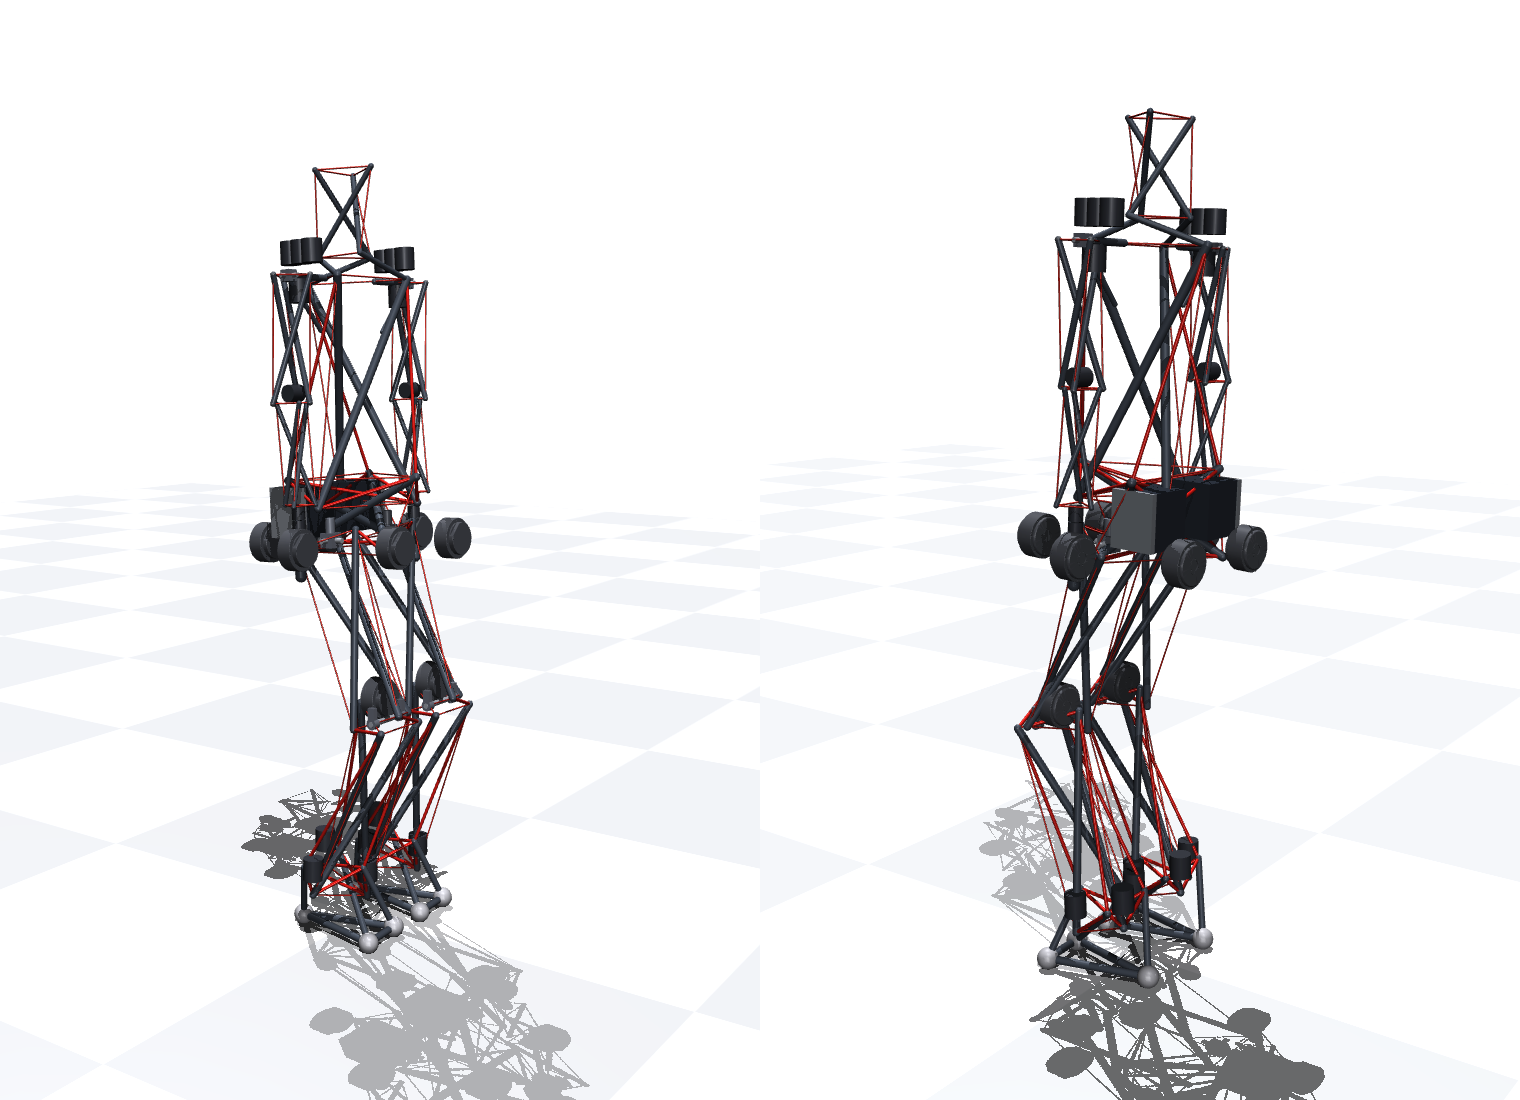
\includegraphics[width=0.99\linewidth]{hybrid_overview.png}
\caption{The hybrid humanoid, front and rear. Every segment is a prism cage;
the six AK70-class hip drives ring the pelvis girdle and the two swappable
battery packs ride posterior rails; XM540-class drives sit on the shank rings
(ankles) and torso (shoulders). White cables are the tensegrity joints at
ankles and waist; steel-grey axles mark the hip gimbals and knee clevises.}
\label{fig:overview}
\end{figure}

\begin{figure}[tb]
\centering
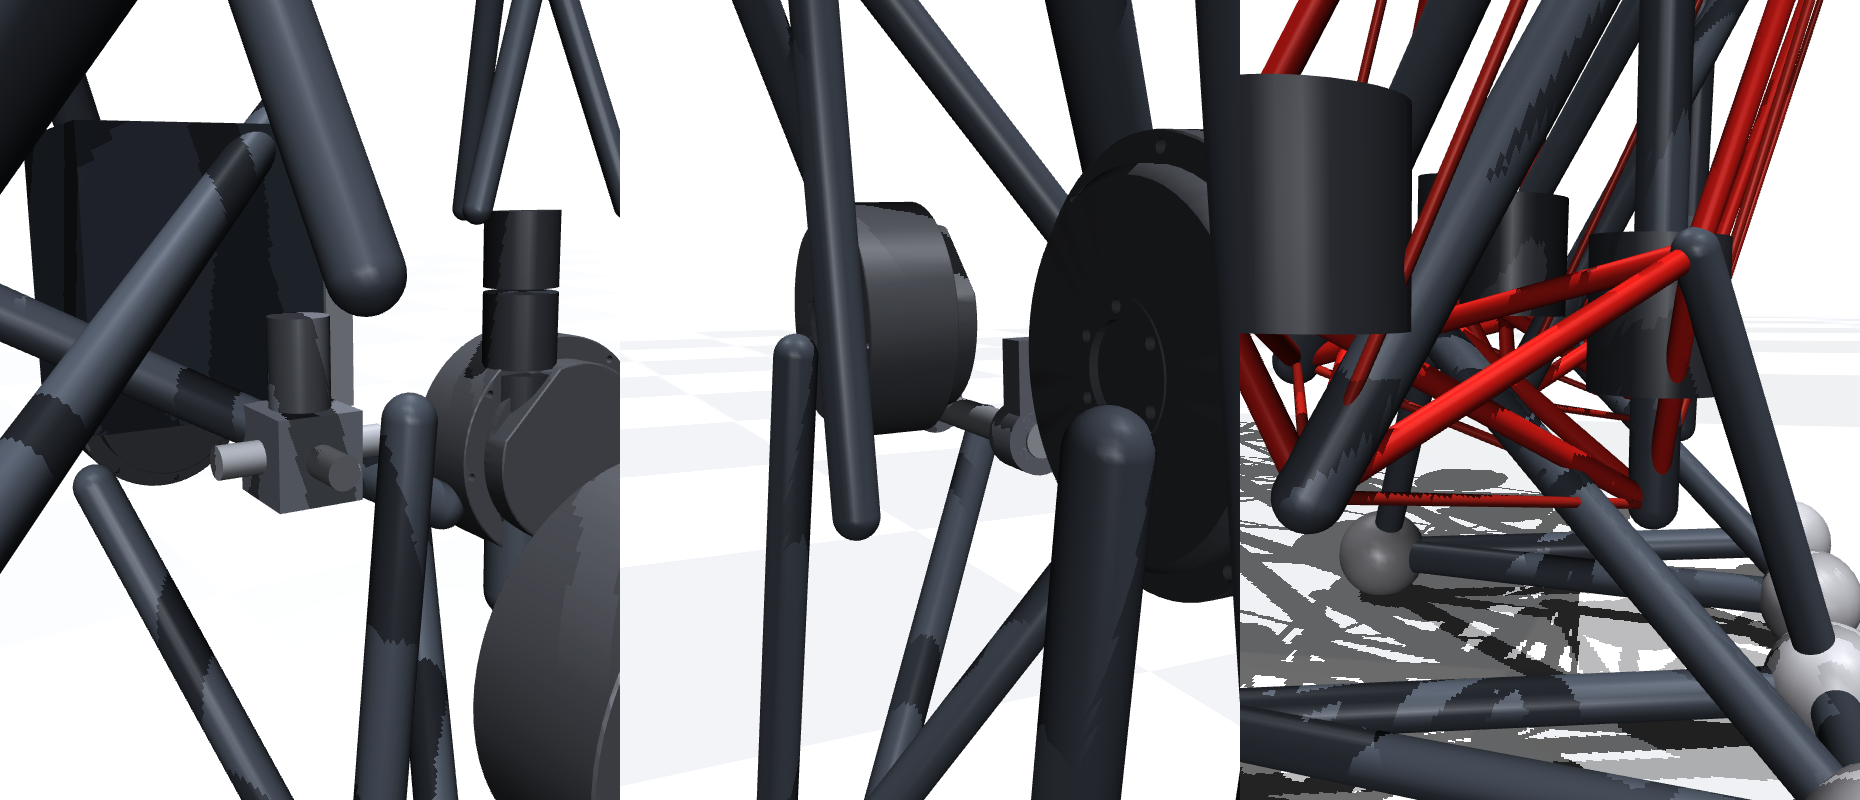
\includegraphics[width=0.99\linewidth]{hybrid_joints.png}
\caption{The three joint types, left to right: hip --- three-axis gimbal
(vertical yaw pivot from the girdle, cross block, roll and pitch axles);
knee --- clevis lugs and steel cross-pin in a bearing pair; ankle --- no
bearing at all: the foot's mast reaches into the shank cage and twelve
counter-wound cables carry the joint.}
\label{fig:joints}
\end{figure}

\begin{figure}[tb]
\centering
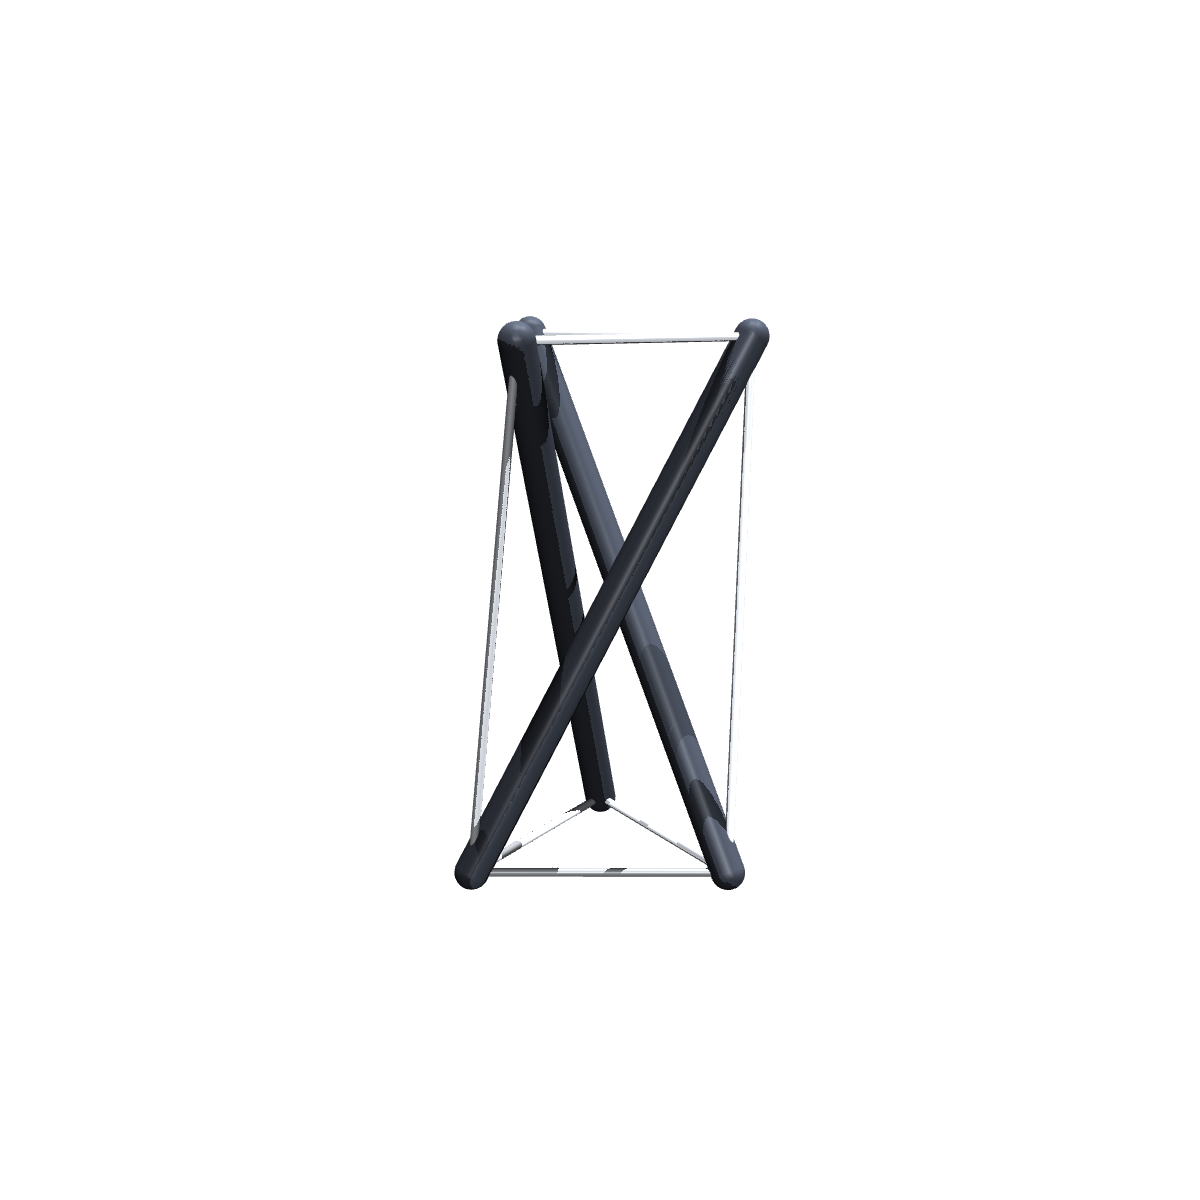
\includegraphics[width=0.52\linewidth]{prism_cell.png}
\caption{The reference cell: a true floating 3-strut tensegrity prism after
dynamic form finding. The three struts (dark) touch nothing; nine tension-only
cables (white) hold the cell at the equilibrium twist of $29.8^\circ$.}
\label{fig:prism}
\end{figure}

\subsection{Physical specification of the members}
\label{sec:members}
Since the structural argument for tensegrity is an argument about members, the
members are specified rather than allowed for. Both families are sized from
the simulated loads (Table~\ref{tab:members}).

\textbf{Struts.} \numStruts{} CFRP tubes, \strutLenMin--\strutLenMax\,mm long,
\strutOdMin--\strutOdMax\,mm outside diameter. The governing axial load is not
cable tension --- resolving the cable tensions along each strut axis over
logged walks gives a peak of only \strutPeakN\,N --- but the ground reaction
entering a cage through its hinge, \strutLoadStumble\,N per strut at a 0.1\,m
stumble landing. Euler sizing with a safety factor of two puts \emph{every}
strut at the thinnest wall we would specify for a bonded joint,
\strutWall\,mm, with worst margin $\strutWorstMargin\times$ on the longest
torso members. The compression network is therefore
manufacturability-limited, not load-limited, at \strutTubeMass\,kg of tube
plus \strutFittingMass\,kg of bonded end fittings.

\textbf{Tendons.} Twelve-strand UHMWPE, sized from the larger of two demands:
the per-cable tension the gait asks for (99th percentile over states, worst
over the payload range, from the unbounded tension distribution of
Sec.~\ref{sec:evidence}) and the pose-independent requirement that one loop
reach its joint's torque limit through the moment arm it has,
$\tau_{\max}/r_{\mathrm{eff}}$. At a safety factor of 3 on breaking load and
0.85 for a buried splice, leg and waist groups take 4\,mm rope
(\ropeBLLeg\,kN), shoulders 2.5\,mm, and the prism-cell cables 1\,mm. Worst
RMS utilisation is \ropeUtilRms\% of breaking load.

The mass result qualifies a common shortcut. The \emph{rope} is grams ---
\ropeMass\,kg for all \numTendonCable{} cables. The \emph{tension network} is
not: its \numCableEnds{} terminations mass \termMass\,kg, seventeen times the
rope they terminate, and the \nodeCount{} node clusters add \nodeMass\,kg.
The declared load path also has to be paid for. Compression runs
strut\,$\rightarrow$\,node\,$\rightarrow$\,hinge\,$\rightarrow$\,node\,$\rightarrow$\,strut,
so each of the \hingeDofCount{} rotational degrees of freedom needs a bearing
pair, clevis and axle sized for the joint reaction rather than for cable
tension --- about \bearingPerDof\,g per degree of freedom at this load, or
\bearingMass\,kg. Members, interfaces and bearings then total
\membersMass\,kg against a 5.9\,kg line, leaving \shellAllowance\,kg for
shell, sewn channels and fasteners, which is not enough. The budget does not
close with hinges in it.

Two conclusions follow. A network of this kind is priced by its interface
count, not its cable count: the rope is \ropeMass\,kg and its terminations,
nodes and bearings are \termMass$+$\nodeMass$+$\bearingMass\,kg. And the
hinge-free geometry of Sec.~\ref{sec:jointcell} is not only a mechanics
argument but a mass argument, since deleting the bearings returns
\bearingMass\,kg --- roughly what the textile shell needs.

\begin{table}[tb]
\centering
\caption{Physical specification of the compression and tension members, sized
from the simulated loads. Strut walls are at minimum manufacturable stock
throughout; rope diameters are set by the loop torque requirement. Masses
include bonded strut end fittings and rope terminations.}
\label{tab:members}
\setlength{\tabcolsep}{4pt}%
\begin{tabular}{@{}llccr@{}}
\toprule
member & spec & $n$ & load & kg\\
\midrule
\multicolumn{5}{@{}l}{\emph{compression, CFRP tube}}\\
thigh, shank & 16--18\,mm $\times$ \strutWall\,mm & 12 & 485\,N & 0.25\\
torso, pelvis & 18--20\,mm $\times$ \strutWall\,mm & 21 & 485\,N & 0.50\\
arm, head, foot & 12--14\,mm $\times$ \strutWall\,mm & 27 & 485\,N & 0.28\\
\midrule
\multicolumn{5}{@{}l}{\emph{tension, 12-strand UHMWPE}}\\
hip, knee, ankle, waist & 4\,mm, \ropeBLLeg\,kN & 54 & 2.4\,kN & 0.50\\
shoulder & 2.5\,mm, 5.0\,kN & 24 & 1.4\,kN & 0.21\\
elbow, wrist, neck & 1.5--2\,mm, 1.8--3.2\,kN & 36 & 0.7\,kN & 0.30\\
prism-cell cables & 1\,mm, 0.8\,kN & 108 & prestress & 0.88\\
\midrule
node clusters & machined, 3 struts each & \nodeCount{} & --- & \nodeMass{}\\
joint bearings & pair $+$ clevis $+$ axle & \hingeDofCount{} & 1.5\,kN &
\bearingMass{}\\
\midrule
members total & & & & \membersMass{}\\
budget line (Table~\ref{tab:mass}) & & & & 5.90\\
\bottomrule
\end{tabular}
\end{table}

\textbf{The stiffness this implies.} A 4\,mm UHMWPE cable on an 87\,mm hip run
has an axial stiffness $EA/L$ of about 7\,MN/m once bedded in; across groups
the specified ropes run \kRopeMin--\kRopeMax\,MN/m. The simulation models
those cables as springs of \kModelMin--\kModelMax\,N/m, a median factor of
\stiffGapRope{} softer, so the modelled network is a rope network in series
with a soft element the model does not name. The specification says what that
element must be. At bare-rope stiffness the 3--4\% prestress the model applies
would be far past breaking load, and setting a useful prestress of a few
hundred newtons would need \takeupMin--\takeupMax\,\textmu m of take-up
resolution at every one of \numTendonCable{} turnbuckles. Interposing a
deliberate series-elastic element of \kSeriesMin--\kSeriesMax\,kN/m makes the
same prestress a millimetre-scale adjustment --- and that range is exactly the
series compliance $k_{\mathrm{ser}}$ the transmission study of
Sec.~\ref{sec:codesign} assumes when computing force bandwidth. The design is
consistent; the model is $\sim$\stiffGapSeries$\times$ softer than even that
element, which is the single largest modelling gap in this work and is
discussed in Sec.~\ref{sec:questions}.

\subsection{Mass budget and batteries}
Two 2.5\,kg packs ride in dovetail rails on the posterior pelvis, below the
waist joint so waist actuators never carry them, symmetric about the sagittal
plane. Two packs are the minimum for live hot-swap: simulated removal of one
shifts the centre of mass by 5.8\,mm laterally, 12\% of a foot half-width, and
both controllers below balance through it without retuning. The pack
specification --- 450\,Wh in 2.5\,kg, i.e.\ 180\,Wh/kg at pack level --- is a
target requiring 250--270\,Wh/kg cells and a light enclosure, at the top of
what current cells deliver. We quote no runtime figure: it is bounded below by
the quiescent draw of \numMotors{} QDD drives holding posture, which is not
negligible and has not been measured.

\begin{table}[tb]
\centering
\caption{Mass budget of the hybrid. Every drive is mounted proximally to the
joint it serves; the two tensegrity joints carry no bearings at all.}
\label{tab:mass}
\setlength{\tabcolsep}{4pt}%
\begin{tabular}{@{}lccl@{}}
\toprule
item & $n$ & kg & where\\
\midrule
hip drives, AK70-class & 6 & 3.1 & pelvis girdle\\
knee drives, AK70-class & 2 & 1.0 & thigh cuffs\\
ankle tension drives, XM540 & 6 & 1.0 & shank rings\\
waist tension drives, XM540 & 6 & 1.0 & torso ring\\
arm drives, XM540/XM430 & 14 & 1.7 & torso + arm\\
articulation hardware (gimbals, clevises) & & 0.8 & hips, knees\\
battery packs, hot-swappable & 2 & 5.0 & pelvis rails\\
compute + power & & 0.5 & pelvis\\
structure: cages, cables, feet, masts & & 6.0 & distributed\\
\midrule
total & & 20.1 & \\
\bottomrule
\end{tabular}
\end{table}

\section{Modelling and Controllability}
\label{sec:model}
The robot is modeled in MuJoCo \cite{todorov2012mujoco} by a parametric
generator emitting two variants from one node graph: a \emph{joint-torque
model} (27 motors at the hinges; the planner's model) and a
\emph{cable-driven model} (\numActuatable{} tension-only actuators). Four
implementation points matter beyond standard MJCF.

\textbf{Cables must be tension-only.} A MuJoCo tendon with a single
\texttt{springlength} is a \emph{bidirectional} spring --- it pushes when
short. Modeled that way, every ``cable'' is secretly a strut and the structure
is fake. All cables therefore use the deadband form
$\texttt{springlength}=[0,\;\ell_0]$, giving
$F=k\max(0,\ell-\ell_0)+c\dot\ell|_{\text{taut}}$ with
$\ell_0=(1-p)\ell_{\text{home}}$ set by the prestress fraction $p$ (4\% at
joints). A second compile pass recomputes $\ell_{\text{home}}$ from the model
itself so that wrapped cables carry the intended prestress.

\textbf{Actuation convention.} Tendon actuators use negative gear
($F=-g\,u$, $u\in[0,1]$, $g=-\Fmax$), making tension-only actuation explicit;
joint motors use $u\in[-1,1]$ with the torque limit in the gear. Normalizing
all controls to $\mathcal{O}(1)$ is required by MJPC, whose exploration noise
and control costs assume unit-scale actions.

\textbf{Capstan drums for long-axis rotation.} A cable helixed around a limb
has a small moment arm about the limb's own long axis (16--25\,mm here), so
yaw DoFs were under-actuated by $1.6$--$2.5\times$ or worse. Each such joint
carries a capstan drum coaxial with its axis, making
the moment arm equal the drum radius (35--55\,mm) independently of cage
geometry. Since one tendon can wrap a geom only once and disengages at some
joint angles, the physical multi-turn winding is modeled as six tendons spaced
around the drum --- still \emph{one} motor in hardware. Wrap engagement is
discontinuous, which destroys the finite-difference derivatives iLQG needs, so
the planner model carries the drum geometry but not the drum cables.

\textbf{Verification pipeline.} Every geometry change is gated by four
automated checks: all cable endpoints on strut tips; the cable-authority
analysis below; a scripted balance test (PD plus a centre-of-mass ankle
strategy, 60\,N forward and 40\,N lateral pelvis pushes) on the joint-torque
model; and the same balance achieved by \emph{pure tension distribution} on
the cable model, solving $\min_{0\le t\le\Fmax}\|Mt-\tau\|^2$ at 250\,Hz. The
last check also produced a hardware requirement: in our zero-order-hold
implementation a 62.5\,Hz tension loop went unstable against the $\sim$15\,Hz
joint-stiffness dynamics while 250\,Hz was stable. A $4\times$ rate ratio is
marginal rather than categorically insufficient, so the reading is that the
tension loop must be designed against these dynamics, not that 62.5\,Hz is a
general bound.



\subsection{Cable authority: the binding constraint}
\label{sec:authority}
With tension-only actuation the achievable torque about DoF $j$ is bounded by
\begin{equation}
  \tau_j^{+} = \sum_c \max(0, M_{jc})\,\Fmax_c,\qquad
  \tau_j^{-} = \sum_c \min(0, M_{jc})\,\Fmax_c,
  \label{eq:authority}
\end{equation}
where $M_{jc}=\partial \ell_c/\partial q_j$ is the moment arm of cable $c$
about joint $j$ and $\Fmax_c$ its tension limit. If either bound is near zero
that DoF is uncontrollable regardless of the controller. Eq.~\eqref{eq:authority}
is the per-DoF projection of a condition the cable-driven parallel robot
community formalised two decades ago: because cables pull only, the achievable
wrench set is the positive span of the individual cable wrenches, and the poses
at which a required wrench set lies inside it form the wrench-feasible
workspace \cite{bosscher2004wrench,gouttefarde2006wrench,gouttefarde2007wfw}.
We claim no novelty for the bound itself. What we take from applying it here is
that a legged tendon-driven machine must be gated on it \emph{as a design
constraint over the trajectory}, not merely checked at one pose --- and
Sec.~\ref{sec:hinge} uses its full six-dimensional form to answer a structural
question the per-DoF projection cannot. Two qualifications
travel with any number Eq.~\eqref{eq:authority} produces, and both matter: it
is evaluated \emph{at a configuration}, since moment arms are functions of
$q$, and \emph{over an actuation set}, since the sum runs only over cables a
motor can tension.

As a design gate the bound earns its place. Evaluating it after every geometry
change caught three genuine errors: hip yaw and wrist had \emph{exactly zero}
authority in one direction because all cable families wound with the same
handedness, so opposite-handed \emph{cw}/\emph{ccw} winding is required for
bidirectional yaw; shoulder roll had $0.15\times$ the required torque because
the shoulder socket sat inboard of the joint axis instead of straddling it;
and ankle cables ran nearly horizontally and saturated at their 1.5\,kN limit
during push recovery, fixed by ending the shank cage higher and moving the
foot nodes to heel/forefoot positions.

As a controllability guarantee the bound is far weaker than the assembly-pose
number suggests, and Table~\ref{tab:authority} gives the honest version. At
the assembly pose with every cable independently driven all 27 DoF are
bidirectional with worst margin $\authHomeAll\times$. Evaluated at poses
sampled from logged gait, still with every cable driven,
\authShortGaitAll{} of 27 DoF fall below their joint-torque limit --- hip
pitch to $\authGaitHip\times$, knee to $\authGaitKnee\times$. Restricting the
sum to the \numDrivenCables{} cables the \numMotors{}-motor bill of materials
can tension leaves \authShortGaitBom{} of 27 short. Two mechanisms produce
this: moment arms shrink away from the assembly pose, and the drum wrap
disengages at some wrist and shoulder angles, which is why those DoFs reach
exactly zero.

This is a design requirement, not a defect of the analysis. For a single loop
to cover 80\,N\,m at the 1.5\,kN cable limit the effective moment arm must be
$\rNeedHip$\,mm; the present cage offers $\rHaveHip$\,mm at hip pitch and
$\rHaveKnee$\,mm at the knee. Closing that gap is the principal geometric
target the loop has produced.

\begin{table}[tb]
\centering
\caption{Cable authority (Eq.~\ref{eq:authority}) depends on where it is
evaluated and on which cables a motor can reach. Entries are the number of
DoFs whose bidirectional authority falls below the joint-torque limit, and the
worst margin over the 27 DoFs.}
\label{tab:authority}
\begin{tabular}{llcc}
\toprule
configuration & actuation set & DoFs short & worst margin\\
\midrule
assembly pose & all cables & \authShortHomeAll{}/27 & $\authHomeAll\times$\\
gait poses    & all cables & \authShortGaitAll{}/27 & $\authGaitAll\times$\\
assembly pose & \numMotors{} loops & \authShortHomeBom{}/27 & $\authHomeBom\times$\\
gait poses    & \numMotors{} loops & \authShortGaitBom{}/27 & $\authGaitBom\times$\\
\bottomrule
\end{tabular}
\end{table}

\section{Predictive Control and Gait Generation}
\label{sec:mpc}

\subsection{Receding-horizon iLQG}
The controller solves, at every replanning instant,
$\min_{u_{0:T-1}}\sum_t \ell(x_t,u_t)$ subject to $x_{t+1}=f(x_t,u_t)$, where
$f$ is the full MuJoCo dynamics and the running cost is a weighted sum of
norms of residuals \cite{howell2022mjpc}. iLQG
\cite{li2004ilqr,tassa2012synthesis} rolls out the current policy, linearizes
the dynamics and quadratizes the cost along the trajectory, performs a
regularized backward Riccati pass yielding a time-indexed affine feedback law
with control limits handled as in \cite{tassa2014control}, and line-searches
the rollout. We use MJPC's asynchronous implementation with horizon 0.6\,s and
planning timestep 20\,ms; the plant integrates at 4\,ms.

Two findings from a headless synchronous replica shaped deployment. Planner
choice is task-dependent: for standing, iLQG keeps balance down to one
planning iteration per 64\,ms of sim time while predictive sampling needs one
per $\sim$12\,ms, and for the \numActuatable-input cable model the situation
reverses. Second, the \numActuatable-dimensional tension space is at the edge
of what direct MPC can carry: the cable model balances only with a planning
iteration every physics step. Both argue for the hierarchical architecture we
use --- plan in 27-DoF joint space, distribute to tensions underneath --- and
for the co-design premise generally, since controller capability is a design
constraint on par with mass.

\subsection{An analytic gait reference}
\label{sec:gait}
Pure cost shaping (reward forward velocity, penalize falling, ``keep feet
moving'') produced only rhythmic stepping in place: across three 14-s trials
net displacement was $-0.32$, $+0.11$ and $+0.77$\,m. Two cost terms were
actively \emph{anti-walking}: a straight-line term pinning the pelvis to
$y=0$, which forbids the lateral weight shift that unloads a foot, and a
capture-point term forever centering the centre of mass between the feet,
which is wrong during single support.

The remedy is to give the optimizer a kinematically consistent reference to
track, generated analytically inside the residual. With gait phase
$\phi=\operatorname{mod}(t f_c,1)$ (a pure function of time, hence identical
in plant and rollouts) and duty factor $d=0.65$: the pelvis tracks a lateral
weight shift $y_{\mathrm{ref}}=A\sin(2\pi(\phi-\phi_0))$, $\phi_0{=}0.07$, so
weight is over each stance foot just before the other lifts; in the pelvis
frame a stance foot slides backward while a swing foot returns with sinusoidal
clearance,
\begin{equation}
x_{\mathrm{f}}(\phi)=
\begin{cases}
\left(\tfrac12-\tfrac{\phi}{d}\right)s, & \phi<d\ \text{(stance)}\\[2pt]
\left(\tfrac{\phi-d}{1-d}-\tfrac12\right)s, & \phi\ge d\ \text{(swing)}
\end{cases}
\end{equation}
with stride $s=v d/f_c$ and lift $z_{\mathrm{f}}=h\sin(\pi(\phi-d)/(1-d))$
(Fig.~\ref{fig:gaitref}), the feet half a cycle apart. The swing-foot landing
point is biased by centre-of-mass velocity error in the manner of Raibert
\cite{raibert1986legged} and the capture point \cite{pratt2006capture},
$\Delta p=\tfrac{T_s}{2}(v-v_d)+k_{cp}(v-v_d)$, ramped in over the swing ---
this is what makes stepping \emph{stabilizing}, since a purely prescribed
pattern moves with the falling body and never steps out to catch it. Foot
targets become references for all twelve leg joints by analytic flat-foot
inverse kinematics (planar two-link solution after hip roll, with
$\theta_{\text{hip}}+\theta_{\text{knee}}+\theta_{\text{ankle}}=0$ enforcing
sole flatness), verified to $<0.1$\,mm against forward kinematics. Arms
counter-swing; posture is referenced to a bent-knee \emph{walk-ready} pose,
because at the assembly pose the legs are fully extended and a posture cost
pulling toward straight knees fights the gait.

\begin{figure}[tb]
\centering
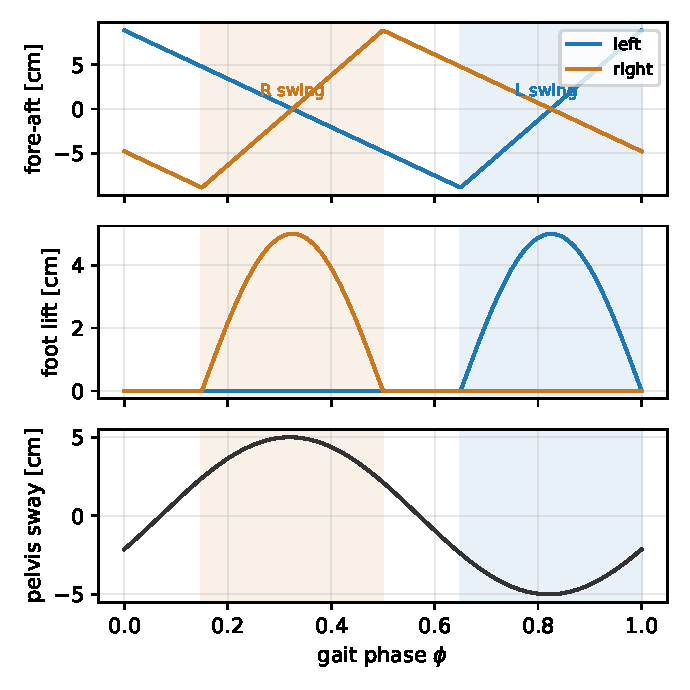
\includegraphics[width=0.86\linewidth]{gait_reference.pdf}
\caption{The analytic gait reference over one cycle ($v=0.3$\,m/s,
$f_c=1.1$\,Hz, duty 0.65): fore--aft foot targets in the pelvis frame (top),
swing clearance (middle), and lateral pelvis sway (bottom). Shaded bands mark
the swing windows of each foot.}
\label{fig:gaitref}
\end{figure}

\subsection{Walking (fully hinged variant)}
The gait machinery was developed and validated on the fully hinged 27-DoF
variant, which is also where every load trace used for dimensioning
originates. With reference tracking, iLQG walks it at
\walkSpeed$\pm$\walkSpeedSd\,m/s in \walkRate{} of ten trials, at a steady
pelvis height of 0.78\,m; the longest logged run covers 6.0\,m in 29\,s. Cost
of transport is \walkCot{}, high for a machine of this mass. The hybrid's own
walking results appear in Sec.~\ref{sec:hybridwalker}.

Three qualifications matter. The success rate is \walkRate{} and not $10/10$:
the gait sits close enough to its stability boundary that planner
stochasticity decides individual trials, which is why every capability claim
below is a rate with a confidence interval. Walking survives a $4\times$
reduction of planning rate (one iteration per 32\,ms of sim time), and the
planner runs at \realtimeFactor$\times$ real time with a 16\,ms planning
interval on a laptop CPU over \realtimeN{} runs --- close to, but not at, real
time. And the result is obtained on the joint-torque model;
Sec.~\ref{sec:evidence} asks separately whether the cables can deliver those
torques.

\section{Simulation-Driven Dimensioning}
\label{sec:codesign}

\subsection{Requirements and transmissions}
Because the verified simulations expose every cable tension, the balance
scenario yields per-joint peak tension, RMS tension, slew, cable velocity and
stroke directly. The ankle emerges as bandwidth-critical (64\,kN/s slew,
$\approx$46\,Hz force modulation) and the hip as stroke-critical (177\,mm).
These are \emph{balance} requirements; the walking traces of
Sec.~\ref{sec:evidence} ask for considerably more tension, and supersede them.

Force control acts through the series compliance $k_{\mathrm{ser}}$ of the
tendon run. A motor with rotor inertia $I_r$ and gear ratio $G$ driving radius
$r$ reflects $m_{\mathrm{eff}}=I_rG^2/r^2$ into the cable, limiting open-loop
force bandwidth to
\begin{equation}
  f_{\mathrm{bw}} = \frac{1}{2\pi}\sqrt{k_{\mathrm{ser}}/m_{\mathrm{eff}}},
  \label{eq:bandwidth}
\end{equation}
with closed-loop feedback buying a further $2$--$3\times$. Small $r$ (spool)
maximizes force and gives unlimited stroke but crushes bandwidth; large $r$
(lever) restores bandwidth at the price of force and a stroke bounded by
$r\Delta\theta$. With vendor data for the CubeMars AK70-10 ($G{=}10$) and
AK60-6 ($G{=}6$), a 12\,mm spool on the AK70-10 delivers 2\,067\,N and
unlimited stroke but only 3.5--9.5\,Hz ($k_{\mathrm{ser}}$ from
40--300\,kN/m), while a 50\,mm lever reaches $\sim$40\,Hz but only 105\,mm of
stroke and 496\,N. The design splits accordingly: \emph{spools} at hips, knees
and waist, where stroke rules and 5--10\,Hz suffices provided tendon runs are
kept short and stiff --- making channel stiffness a first-class textile
requirement; \emph{lever arms} with a larger AK10-9-class motor at the ankles;
and \emph{drums} wherever the axis itself is the problem.

\subsection{From cables to motors, and the shortfall}
The tension network is deliberately rich (\numActuatable{} actuatable joint
cables), but a cable is grams of rope where a motor is 0.3--0.96\,kg; driving
every cable would put \allMotorMass\,kg of motors on a 27.6\,kg robot. Three
mechanisms collapse the count: a \emph{loop drive} (one motor, double-wound
spool paying out one cable while hauling its antagonist) gives bidirectional
torque per DoF from one motor and two cables; undriven cables remain
load-bearing as \emph{passive prestress elements} (spring plus turnbuckle,
\numPassiveCables{} of \numActuatable{}); and antagonist
\emph{co-contraction pairs} are added only where variable stiffness earns its
mass, at waist and shoulders. The result is $27+9=\numMotors{}$ motors driving
\numDrivenCables{} cables at \bomMass\,kg.

\textbf{This bill of materials does not meet its own torque specification, and
the reason is geometric.} A single loop delivers $\Fmax\,r_{\mathrm{eff}}$
about its DoF: at the assembly pose that is \singleLoopHip\,N\,m at hip pitch
and \singleLoopKnee\,N\,m at the knee against an 80\,N\,m requirement, and
Table~\ref{tab:authority} shows the shortfall widening over the gait. Two
remedies exist and they are not equivalent. A second loop where one is short
(hip pitch, knee, elbow, waist roll) costs seven motors and
$+\extraMotorMass$\,kg, raising the actuator budget to \bomMassFixed\,kg, but
does not help where the gait-wide margin is zero, because a second cable of
the same family loses its moment arm at the same poses. Enlarging the cage so
that $r_{\mathrm{eff}}\ge\rNeedHip$\,mm at hip pitch and knee costs no motors
at all. The measurement therefore does not merely flag a shortfall; it says
which design change to make.

\section{Experimental Evidence}
\label{sec:evidence}
All experiments run against a \emph{rigid-equivalent baseline} --- the same
27-DoF model with the tension network removed --- with actuation held constant
across arms of every comparison, so that only the structural paradigm varies.
Walking conditions use $n=10$ trials and are reported as success rates with
Wilson 95\% intervals, because iLQG success near the stability boundary is
stochastic. Table~\ref{tab:experiments} summarises protocols and results;
Figs.~\ref{fig:experiments}--\ref{fig:tradecurves} give the data. Every number
is regenerated from the logged runs by the analysis scripts and injected into
this text as a macro, so prose and data cannot drift.

\textbf{E1, impact tolerance.} Unpowered drops from 0.05--1.0\,m in the cross
of \{cables, no cables\}$\times$\{servo-held, limp\}
(Fig.~\ref{fig:experiments}a). Holding actuation constant, the tension network
makes impacts \emph{worse}: at the 0.1\,m stumble height the limp tensegrity
peaks at \eOnePassiveTsgStumble\,N against \eOnePassiveRigidStumble\,N for the
limp rigid equivalent (\eOneDeltaPassiveStumble\%), and at 1\,m
\eOnePassiveTsgCrash\,N against \eOnePassiveRigidCrash\,N
(\eOneDeltaPassiveCrash\%). Servo-held against servo-held the network is
neutral (\eOneDeltaHeldStumble\% at 0.1\,m, \eOneDeltaHeldCrash\% at 1\,m).
All \eOnePassiveFell{} of \eOnePassiveN{} limp-tensegrity drops end with the
robot on the floor. The mechanism is the load path: an impulse at the foot
reaches the pelvis through hinges, which do not stretch, so the elastic
network is loaded in parallel with a stiff path rather than in series with it.
Prestress does preserve posture after impact --- at 1\,m the
$3\times$-prestress robot ends higher than the nominal one --- but that is a
different claim from attenuation.

The result is not an artefact of the soft cables the campaign was run with.
Repeating the matched drops with the network replaced by a series-elastic
element per group and prestress specified as a tension (Sec.~\ref{sec:members})
makes it considerably worse: the limp tensegrity then peaks
\physOneLimpTen\% above the limp rigid equivalent at 0.1\,m and
\physOneLimpHundred\% above it at 1\,m, and even the servo-held comparison goes
from neutral to \physOneHeldHundred\% at 1\,m. A stiffer network transmits an
impulse more directly, so the conclusion strengthens with realism rather than
depending on the modelling choice.

\textbf{E2, stiffness.} Endpoint stiffness of the unpowered arm, measured
differentially with a \stiffProbe\,mN probe about the settled pose;
deflections stay in the millimetre range and halving the probe changes the
result by \stiffLinearity\%, confirming the linear regime. The cable network
raises lateral endpoint stiffness from \stiffNoCables\,N/m with cables removed
to \stiffZeroPre\,N/m with cables present but \emph{untensioned} --- a factor
of \stiffCablesRatio{} that is pure kinematic constraint. Sweeping assembly
prestress from $0$ to $5\times$ then moves it only between \stiffPreLo{} and
\stiffPreHi\,N/m, non-monotonically (Fig.~\ref{fig:experiments}b). Repeating the sweep at
series-elastic stiffness changes the numbers but not the conclusion: the
cables then raise lateral endpoint stiffness from \physTwoNoCables{} to
\physTwoZeroPre\,N/m by their presence alone, a factor of
\physTwoCableRatio{}, and prestress beyond the level needed to take up slack
moves it by \physTwoEngaged\% (\physTwoNominal{} at nominal,
\physTwoHigh\,N/m at $4\times$).

The mechanism is not the hinge. Sec.~\ref{sec:prestressscaling} repeats the
sweep on a hinge-free joint and finds the same flatness, and identifies the
governing quantity: the tangent stiffness of a prestressed network is an
elastic term of order $EA/L$ plus a geometric term of order $T/L$, and
prestress tunes stiffness only when the two are comparable. At the rope
stiffness this design specifies, the geometric term is
\jointGeomElasticRope\% of the elastic one. What does modulate stiffness is
\emph{differential} tension: shoulder co-contraction takes lateral endpoint
stiffness from \stiffCoLo{} to \stiffCoHi\,N/m ($\stiffCoRatio\times$) with no
added hardware, saturating early at \stiffCoKnee\,N/m by 50\,N, so the useful
operating range is tens of newtons.

\textbf{E3, graceful degradation.} Severing a cable removes both its actuator
and its passive spring. All \eThreeSinglesOk/\eThreeSinglesN{} single cuts
survive standing plus a 40\,N push, including the worst-authority cable in the
network. Randomly chosen multi-cable failures survive at every level tested:
\eThreeRandTwo, \eThreeRandFour{} and \eThreeRandEight{} for $k=2,4,8$ drawn
from the whole network, and \eThreeLegTwo, \eThreeLegFour, \eThreeLegEight{}
restricted to leg and waist cables. Random draws are a weak adversary,
however, since most of the network is arm and neck cable that quiet standing
never loads. Selecting the $k$ cables that most reduce the worst per-DoF
authority margin and testing against four push directions, the robot survives
\eThreeAdvTwo{} at $k=2$ and \eThreeAdvFour{} at $k=4$, and fails
\eThreeAdvEight{} at $k=8$ --- three hip, three knee and two ankle cables on
one leg. The bounded statement: no single cable is structural, random loss of
up to eight is tolerable, a targeted loss of eight is not.

\textbf{E4, proximal mass placement.} Moving knee, ankle and arm motor masses
from their proximal mounts to the joints they drive, with identical totals,
degrades the same controller from \walkRate{} successful walks at
\walkSpeed\,m/s to \distalRate{} at \distalSpeed\,m/s
(Fig.~\ref{fig:experiments}d). This is the property tendon transmission buys,
and it is measurable rather than merely elegant.

\textbf{E5, tendon realisability.} Every walking result above is produced on
the joint-torque model, whose motors deliver their limits at every pose.
Mapping the logged walking torques through the bounded tension distribution
$\min_{0\le x\le 1}\|M(q)x-\tau\|^2$ shows the network reproduces the demanded
torques exactly for most of the stride --- median residual below
$10^{-3}$\,N\,m --- with concentrated failures: at least one cable is pinned
at the 1.5\,kN bound in \tensSatPct\% of sampled states at zero payload,
rising to \tensSatFour\% at 4\,kg and \tensSatTwenty\% at 20\,kg, leaving up
to \tensResidTwelve\,N\,m of demanded joint torque undelivered. Lifting the
bound, the gait asks for \tensNeeded\,N of peak cable tension, roughly
$1.6\times$ the specified rating, and the busiest cable runs at
\tensBusiestRms\,N RMS --- about two thirds of its working load continuously,
which is a fatigue rather than a strength problem.

Whether a gait exists \emph{inside} the achievable set is a different question
from whether this gait does, so we re-ran the planner on models whose joint
torque limits were capped at the tendon-achievable envelope of
Table~\ref{tab:authority}. \eSixSummary{} This separates the two candidate
causes cleanly and is the most useful single result of the campaign: the
topology can support a gait, the actuation set as specified cannot deliver
one.

\textbf{Payload and speed.} The fully hinged machine's capability envelope,
measured at $n=10$ per point, provides the comparison endpoint for the
hybrid's envelope in Sec.~\ref{sec:hybridenvelope}
(Fig.~\ref{fig:sweeps}). Trunk boxes of 2--20\,kg give success rates
\cpayTwoRate{} through \cpayTwentyRate{} with speed falling from \cpayTwoV{}
to \cpayTwentyV\,m/s --- flat in payload to within the Wilson intervals
(pooled \cpayAllPct\%, \cpayAllCiLo--\cpayAllCiHi\%), so this design's trunk
payload limit was never found; placement matters more than magnitude (a rear
backpack mount at $-16$\,cm gives \rpaySixteenRate{} at 16\,kg against
\cpaySixteenRate{} centred). The tendon side is what binds: at 20\,kg the
tension distribution is pinned against the cable limit for \tensSatTwenty\%
of the stride. A box held under one hand with the arm PD-held saturates the
30\,N\,m shoulder-pitch motor at 5\,kg while the busiest shoulder cable
carries 307\,N of its 700\,N limit, so arm payload is \emph{motor}-limited,
not tendon-limited. Commanded speeds of 0.10--0.45\,m/s show no cliff:
reliability degrades smoothly through \spdTwentyRate{}, \spdThirtyRate{},
\spdThirtyFiveRate{}, \spdFortyRate{} and \spdFortyFiveRate{} while achieved
speed rises from \spdTwentyV{} to \spdFortyFiveV\,m/s (the grey curve of
Fig.~\ref{fig:sweeps}a).

\subsection{Requirement trade curves}
\label{sec:sweep}
Fig.~\ref{fig:tradecurves} plots what an outer design loop would consume: peak
and RMS joint torque per leg group, and peak required cable tension, against
commanded speed and carried mass. Each point is one pass of generator
$\rightarrow$ authority check $\rightarrow$ headless plan-and-act harness
$\rightarrow$ requirement extraction. Two features are design-relevant. Peak
joint torque is saturated against its limit across the whole range, so these
curves report what the design \emph{allows} rather than what the gait
\emph{needs} --- the signature of an under-dimensioned actuation set. Peak
required cable tension is not saturated by construction and rises from
\tensNeeded\,N at zero payload; it is the quantity that should size the next
iteration's cable and moment arm.

\begin{figure}[tb]
\centering
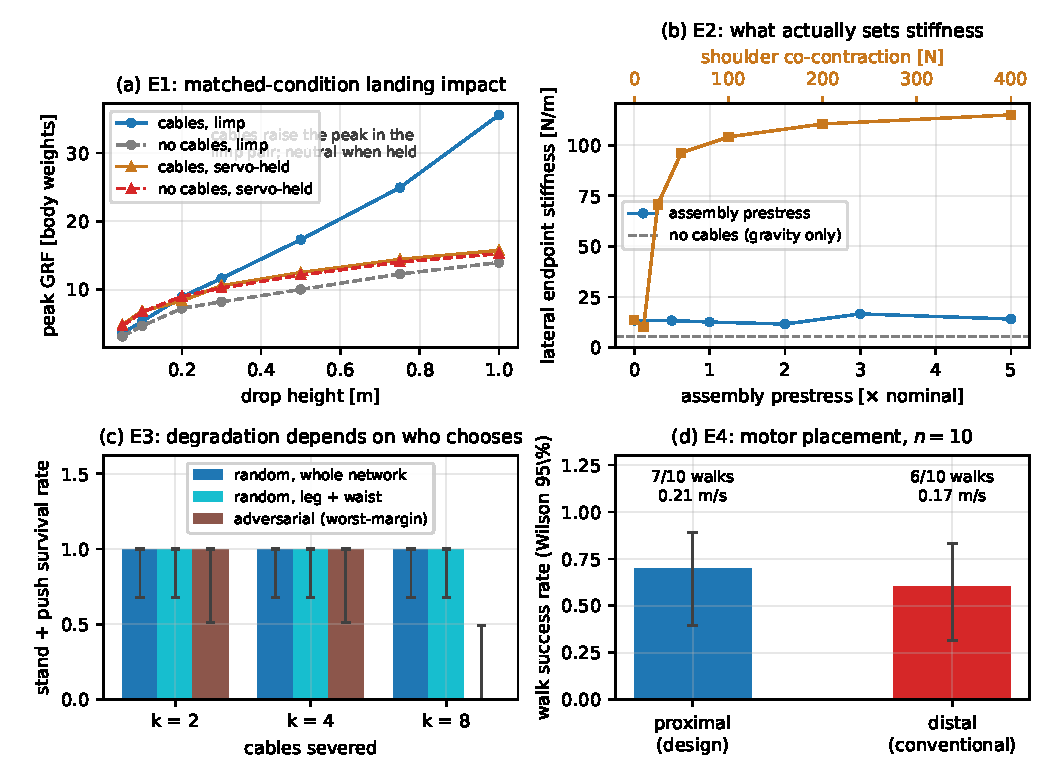
\includegraphics[width=0.95\linewidth]{experiments.pdf}
\caption{(a) E1: peak ground reaction in a 250\,ms landing window vs.\ drop
height; the matched pairs (limp vs.\ limp, held vs.\ held) are what the claim
rests on. (b) E2: lateral hand endpoint stiffness vs.\ assembly prestress
(blue, bottom axis) and vs.\ shoulder co-contraction (orange, top axis).
(c) E3: stand survival under severed cables, random vs.\ adversarial
selection. (d) E4: proximal vs.\ distal motor placement, $n=10$.}
\label{fig:experiments}
\end{figure}

\begin{figure}[tb]
\centering
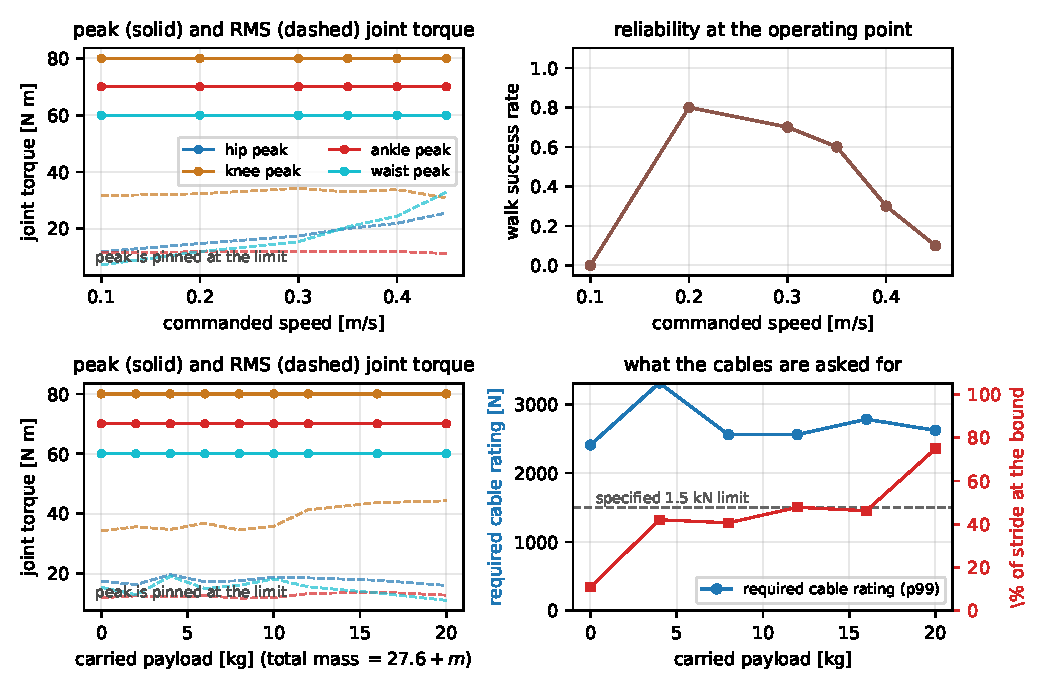
\includegraphics[width=0.98\linewidth]{tradecurves.pdf}
\caption{Requirement trade curves extracted automatically from the same runs:
peak and RMS leg-group joint torque and peak required cable tension vs.\
commanded speed (top) and vs.\ total carried mass (bottom). Joint torque is
saturated against its limit throughout.}
\label{fig:tradecurves}
\end{figure}

\begin{table*}[tb]
\centering
\caption{Experiments against the rigid-equivalent baseline, actuation held
constant. Walking conditions are $n=10$.}
\label{tab:experiments}
\begin{tabular}{llp{4.6cm}p{5.6cm}}
\toprule
id & property tested & protocol & result\\
\midrule
E1 & impact tolerance & drops 0.05--1\,m; \{cables, none\}$\times$\{held,
limp\}; matched pairs &
network raises peak reaction at every height
(\eOneDeltaPassiveStumble\% limp at 0.1\,m, \eOneDeltaPassiveCrash\% at 1\,m;
\physOneLimpTen\% and \physOneLimpHundred\% at physical cable stiffness)\\
E2 & stiffness on demand & \stiffProbe\,mN differential endpoint probe;
prestress $0$--$5\times$; co-contraction 0--400\,N &
assembly prestress does not modulate stiffness
(\stiffPreLo--\stiffPreHi\,N/m); co-contraction does,
\stiffCoLo$\to$\stiffCoHi\,N/m ($\stiffCoRatio\times$)\\
E3 & graceful degradation & sever $k$ cables (random and adversarial), stand
$+$ push, 4 directions &
\eThreeSinglesOk/\eThreeSinglesN{} singles and all random $k\le8$ survive;
adversarial $k{=}4$ survives, $k{=}8$ fails\\
E4 & proximal mass placement & motors moved to the joints they drive, same
totals, $n=10$ &
\distalRate{} vs \walkRate{} successful walks; \distalSpeed{} vs
\walkSpeed\,m/s\\
E5 & tendon realisability & Eq.~\eqref{eq:authority} over gait poses and over
the BOM actuation set; re-plan inside the achievable envelope &
\authShortGaitBom{}/27 DoFs short; gait exists for the full network
(\eSixtendonallRate{}) but not for the BOM (\eSixtendonbomRate{})\\
E6 & member sizing & axial loads resolved from cable tensions; CFRP tube and
UHMWPE rope specification &
struts not buckling-critical ($\strutMarginStumble\times$ at a stumble);
members and interfaces \membersMass\,kg\\
E7 & are the joints hinge-free? & kinematic audit; wrench-closure LP per
joint; remove all hinges &
\hingeDof{} hinge DoF, all 3 translations constrained per joint;
\wcThree/\wcTotal{} joints held by cable; hinge-free robot collapses\\
E8 & hinge-free joint & overlapping floating-strut testbed; drop against a
mass-matched pin joint; prestress $\times$ cable stiffness &
force closure from \jointOverlapFrac$H$; impact
$-\jointImpactLo$ to $-\jointImpactHi$\%; prestress ratio
$\jointPreRatioSoft\times$ soft, $\jointPreRatioRope\times$ at rope\\
P & payload and speed & trunk box 2--20\,kg; speed 0.10--0.45\,m/s; $n=10$ &
no payload limit found to 20\,kg; reliability degrades smoothly with speed\\
\midrule
E9 & structural mass parity & rigid frame sized to the same loads (planned) &
---\\
E10 & contact safety & 1\,m/s limb collision (planned) & ---\\
E11 & fatigue, channel stiffness & bench (planned) & ---\\
\bottomrule
\end{tabular}
\end{table*}

\section{The Hinge-Free Joint}
\label{sec:jointcell}
Sec.~\ref{sec:hinge} establishes that this design's joints are bearings and
that its cables could not replace them. This section asks the design question
that follows --- what geometry \emph{would} let cables carry a joint --- and
then uses that geometry as a testbed for the two properties the hinged machine
fails to deliver. The testbed is deliberately small: a proximal cage fixed to
ground, a distal cage of three free-floating struts, a 1\,kg distal payload,
and cables. Nothing touches anything.

\subsection{Overlap is what closes the wrench set}
The failure in the humanoid is that adjacent cages meet end to end, so every
crossing cable pulls the distal cage toward the proximal one. In a tensegrity
tower the stages instead \emph{overlap}: the distal cage's bottom ring sits
below the proximal cage's top ring, so the interface carries a downward-outward
cable family as well as an upward one, and the positive span closes without any
strut touching another.

Sweeping the overlap confirms it (Table~\ref{tab:jointcell}). At zero overlap
there is no closure in any direction and the joint collapses under its own
payload. From \jointOverlapFrac$\,H$ of overlap --- \jointOverlapMm\,mm on a
300\,mm cell --- the interface achieves \emph{force} closure and the joint
carries its load, with tip sag falling as overlap grows.

Full wrench closure ($t_6>0$) is a separate requirement, and an earlier
version of this analysis dismissed it as undesirable --- ``a joint that
resisted every moment would be rigid.'' That reading is wrong, and attempting
to control the force-closed joint exposed why. $t_6=0$ does not mean the
joint is conveniently free about its axis; it means the cable set has
\emph{no self-stress}, therefore no co-contraction state, and \emph{zero
moment authority about at least one axis} --- tension-only actuators can then
only add load to an equilibrium, never oppose a disturbance, and no balance
controller can exist for the joint. A controllable joint needs $t_6>0$, with
the actuators choosing how much moment to exert, including none. The single
cross family used here winds one way and cannot do it; adding the
counter-wound mirror family closes the wrench set at the same cable count ---
the same opposite-handedness rule the yaw drums of Sec.~\ref{sec:model}
required, which we failed to recognise as general. With the counter-wound
pair the joint carries load, has $\ge1.3$\,kN of available co-contraction,
and a chain of them stands passively; force closure alone gives a structure
that stands but cannot be actuated.

\begin{table}[tb]
\centering
\caption{Overlap sweep on the hinge-free joint testbed. $t_3$ and $t_6$ are
the force- and wrench-closure margins of the interface linear program. Force
closure is the criterion: full wrench closure would mean the joint cannot
rotate.}
\label{tab:jointcell}
\begin{tabular}{@{}ccccl@{}}
\toprule
overlap / $H$ & $t_6$ & $t_3$ & tip sag (mm) & verdict\\
\midrule
0.0 & 0 & 0 & 97 & collapses\\
0.1 & 0 & 1.0 & 70 & collapses\\
0.2 & 0 & 1.0 & 49 & force closure, holds\\
0.3 & 0 & 1.0 & 37 & force closure, holds\\
0.4 & 0 & 1.0 & 29 & force closure, holds\\
0.5 & 0 & 1.0 & 23 & force closure, holds\\
\bottomrule
\end{tabular}
\end{table}

\subsection{Impact tolerance returns when the hinge goes}
\label{sec:jointimpact}
Dropping the testbed onto a floor, against a mass-matched control in which the
distal cage is one rigid body on a ball joint --- the bearing this design
currently uses --- gives the comparison the humanoid could not:

\begin{center}
\begin{tabular}{@{}cccc@{}}
\toprule
drop (m) & cable joint & pin joint & difference\\
\midrule
0.05 & \jointImpactCableFive\,N & \jointImpactPinFive\,N &
$-\jointImpactDeltaFive$\%\\
0.10 & \jointImpactCableTen\,N & \jointImpactPinTen\,N &
$-\jointImpactDeltaTen$\%\\
0.20 & \jointImpactCableTwenty\,N & \jointImpactPinTwenty\,N &
$-\jointImpactDeltaTwenty$\%\\
\bottomrule
\end{tabular}
\end{center}

The hinge-free joint attenuates peak ground reaction by
\jointImpactLo--\jointImpactHi\% at every height, consistently and
monotonically, where the hinged humanoid \emph{raises} it by
\physOneLimpTen--\physOneLimpHundred\% (Sec.~\ref{sec:evidence}). Both are
mass-matched and both were settled before release. This is the mechanism
stated in Sec.~\ref{sec:evidence} confirmed by construction: a bearing puts
the elastic network in parallel with a stiff path, and an impulse takes the
stiff path; remove the bearing and the network is in series with the load,
which is the arrangement the tensegrity-lander results
\cite{sabelhaus2015superball,caluwaerts2014design} rely on. Impact tolerance
is available to this architecture. It is simply not available to a hinged
implementation of it.

\subsection{Prestress-tunable stiffness is a materials condition, not a
topology one}
\label{sec:prestressscaling}
The hinge-free testbed also settles the second failed property, and the answer
is not the one the hinge explanation would predict. The tangent stiffness of a
prestressed network is an elastic term of order $EA/L$ plus a geometric term
of order $T/L$; prestress tunes stiffness only when the two are comparable.
Sweeping prestress at three cable stiffnesses on the \emph{same} hinge-free
geometry:

\begin{center}
\setlength{\tabcolsep}{3pt}%
\begin{tabular}{@{}lccc@{}}
\toprule
cable & geom./elastic & $k$, 25--400\,N & ratio\\
\midrule
2\,kN/m (as modelled) & $\le\jointGeomElasticSoft$\% & 20--455\,N/m &
$\jointPreRatioSoft\times$\\
40\,kN/m (series-elastic) & $\le3.3$\% & 15--20\,N/m &
$\jointPreRatioSeries\times$\\
600\,kN/m (near-rope) & $\le\jointGeomElasticRope$\% & 14--14\,N/m &
$\jointPreRatioRope\times$\\
\bottomrule
\end{tabular}
\end{center}

Removing the hinge does \emph{not} restore prestress-tunable stiffness. What
governs it is the ratio of the geometric to the elastic term, and at the rope
stiffness this design actually specifies that ratio is
\jointGeomElasticRope\%. The cell-scale demonstration that motivated the claim
worked only because those cables were modelled at 2\,kN/m, where the geometric
term reaches \jointGeomElasticSoft\% of the elastic one. To make prestress a
useful stiffness control at humanoid scale one would have to run the cables at
a large fraction of breaking load, or deliberately soften them --- which is a
materials and series-elasticity decision, not a topology decision, and it
trades directly against the force bandwidth of Eq.~\eqref{eq:bandwidth}.

\subsection{Does it compose into a whole humanoid?}
\label{sec:cellgraph}
A joint that works in isolation is not a robot. We therefore generated the
entire machine as a graph of cells --- no hinges, no bearings, nothing
touching --- from one description: a list of prism cells and a list of
overlapping ring interfaces. It composes, with one structural qualification
and one hard requirement.

\textbf{Limbs compose linearly.} A chain of $N$ overlapping cells keeps force
closure at every interface and stands, with droop growing linearly at about
\cellChainPer\,mm per cell (\cellChainDroop\,mm at \cellChainMax{} cells). A
pelvis girdle carrying two three-cell legs --- \lbStruts{} floating struts and
\lbCables{} cables --- holds with \lbDroop\,mm of droop and force closure at
both feet, so branching does not break it either.

\textbf{Junctions cannot be cells.} A 3-strut prism has two node rings and can
therefore host at most two interfaces, while a pelvis needs three and a torso
four. Junctions must be multi-ring girdles, and at a girdle three or more
struts meet at each node: they are class-$k$ tensegrity elements, rigid strut
clusters rather than floating cells. The resulting machine is not uniform. Of
\cgStruts{} struts, \cgCellStruts{} float in limb cells and
\cgClusterStruts{} are welded into two rigid junctions at pelvis and torso.
Whether a genuinely class-1 junction exists --- some arrangement in which the
trunk struts also float --- we do not know, and it is the sharpest open
structural question this work produces.

\textbf{Prestress, not geometry, is the binding requirement.} The complete
body --- \cgStruts{} struts, \cgCables{} cables, \cgDof{} floating degrees of
freedom, feet anchored --- stands under its own weight, settling
\cgSettle\,mm at the crown. It does not stand under the machine's payload. At
the 120\,N prestress that suffices for a single joint it collapses with
\cgLoadFail\,kg on the torso vest, and the motors, batteries and compute that
must ride there come to 22\,kg. Sweeping prestress at that load, the structure
requires \cgPreNeeded\,N per cable, at which it settles \cgPreSettle\,mm and
stands. That is a real design number and it propagates: \cgPreNeeded\,N of
prestress needs cell cables rated at 3\,kN rather than the 0.8\,kN of
Table~\ref{tab:members}, and it puts up to \cgNodeLoad\,N of resultant load
into a strut cluster --- still $\cgNodeMargin\times$ inside the critical load
of the 0.5\,mm-wall tube specified there, so the compression members survive
it.

The answer to ``can the whole robot be a graph of tensegrity cells'' is
therefore yes, structurally, at a cost that is now quantified: overlap every
interface, accept rigid junctions at pelvis and torso, and carry an order of
magnitude more prestress than a single cell needs. What we have not shown is
that such a machine can be controlled --- see Sec.~\ref{sec:questions}, where
the \cgDof{} floating degrees of freedom replace the 27-DoF abstraction that
every controller in this paper depends on.

The design conclusion from this section is therefore split. Impact tolerance
is recoverable and costs a geometry change: overlap the cages by at least
\jointOverlapMm\,mm and delete \hingeDofCount{} bearings, which also returns
the \bearingMass\,kg of Table~\ref{tab:members}. Prestress-tunable stiffness
is not recoverable at any topology with high-modulus rope, and variable
stiffness should be budgeted as an actuation cost (co-contraction) rather than
an assembly parameter.

"""
\section{The Hybrid Walker}
\label{sec:hybridwalker}
The preceding sections leave a specific design prescription: hinges where
torque is king, tensegrity where compliance is king. This section reports the
machine built to that prescription, and the result that it walks.

\subsection{Architecture}
The hybrid humanoid (Fig.~\ref{fig:sequence}) is 1.68\,m and
\hybridMass\,kg. Hips (3\,DoF) and knees (1\,DoF) are mechanical hinges with
joint drives --- these joints need 40--80\,N\,m of precisely phased torque,
which is what bearings are for, and their drives are AK70-10-class units
mounted proximally on the pelvis girdle and thigh cuffs. The bearings
themselves are modelled and massed rather than left implicit, closing the
accounting gap the fully hinged design had: each knee is an alloy-steel
clevis pin in a 61802-class bearing pair (\hybridKneeHw\,g), each hip a
three-axis gimbal --- yaw pivot into the girdle, cross block, roll and pitch
axles (\hybridHipHw\,g) --- all sized at a safety factor of 2.3 against the
1.5\,kN stumble reaction. Articulation hardware totals \hybridJointHw\,kg,
against the 1.89\,kg the 27-hinge design required: confining bearings to the
eight DoF that need them returns most of that mass. The ankles are
genuine tensegrity joints: each foot is a tri-pad plate (heel and two
forefoot corners, the anthropomorphic node placement of
Sec.~\ref{sec:design}) carrying a mast whose top ring overlaps into the shank
cage, joined by the counter-wound ABCD cable families of
Sec.~\ref{sec:jointcell} --- twelve cables, no bearing, force and wrench
closure by construction. The ankle drives are XM540-class tension actuators
on the shank ring, sized by the moment-authority argument of
Sec.~\ref{sec:codesign}: at a hinge-free joint the cables act at the cage
radius rather than through a 37\,mm effective arm, so the same joint moment
costs an order of magnitude less tension, and 0.165\,kg drives replace
0.96\,kg ones. The arms are 7\,DoF each --- a three-axis shoulder gimbal, elbow, and
three-axis wrist --- with all seven drives massed and drawn (XM540-class
shoulder cluster mounted proximally on the torso, XM430-class elbow and
wrist). While walking, the planner commands only the two swing DoF per arm;
the other five hold position on their servos' stiffness, which is modelled as
joint stiffness rather than left implicit. The neck is welded. The waist is the second tensegrity joint: the torso is a free body
whose cage nests into the pelvis girdle on the same counter-wound interface
as the ankles, with six of its twelve cables actuated. Walking, the torso
rides the waist cables within $\pm2^\circ$ of level while sagging 2\,cm ---
passive attitude compliance where a rigid spine would transmit every impact.
The two 2.5\,kg battery packs of Sec.~\ref{sec:design} return as swappable
bodies on posterior pelvis rails; pulling one (an asymmetric 2.5\,kg change)
leaves the gait intact with no retuning, transferring the hot-swap result to
the hybrid. The feet and torso are free bodies: nothing kinematic connects
them to the rest of the robot.

\subsection{What it took to walk}
The controller is the analytic-gait-reference iLQG task of
Sec.~\ref{sec:mpc}, with the ankle rows of the posture reference deleted ---
the feet are steered indirectly, through the cartesian gait cost and the
cable coupling. Three findings from making it work are worth recording.

\textbf{Passive ankles do not walk, and the failure is informative.} With the
ankle cables passive, every configuration tested fails identically: the
planner refuses to lift the swing foot. The mechanism is the one
Sec.~\ref{sec:buys} predicts --- without ankle actuation there is no
centre-of-pressure control, so the planner cannot unload a foot except by
whole-body sway, and lifting a loaded foot means lifting the robot. The
refusal is rational. Widening the ankle mast and stiffening its cables
(raising passive roll stiffness toward the lateral toppling rate) does not
change the outcome.

\textbf{The A/B that isolates it.} Welding the feet to the shanks --- same
model, same residual, same costs --- walks immediately and cleanly at
0.18\,m/s. The pipeline was never the problem; the passive ankle was.

\textbf{Actuating the ankle cables recovers walking.} Giving the planner
tension actuators on the A and B cable families (twelve controls, ctrl
$\in[0,1]$, the tension-only convention of Sec.~\ref{sec:model}) produces
walking at \hybridSpeed\,m/s with the pelvis steady to within $\pm$1.5\,cm
--- at a running cost \emph{below} the welded control, because the planner
exploits the compliance it now commands: tensioning the A family lifts the
hanging foot for swing clearance, tensioning B pitches the toe up, and
differential tension steers the landing. The tensegrity ankle is not a
handicap to be tolerated; actuated, it is the better ankle. The duty numbers
say the sizing is right: over the gait the hip and knee motors average
\hybridJointDuty\% of their torque limits and the ankle tension actuators
\hybridAnkleDuty\% of theirs, with brief \hybridAnklePeak\,N peaks at foot
lift --- inside the XM540-class rating that the moment-authority argument
selected, and an order of magnitude below what the hinged design's ankle
demanded.

\begin{figure*}[tb]
\centering
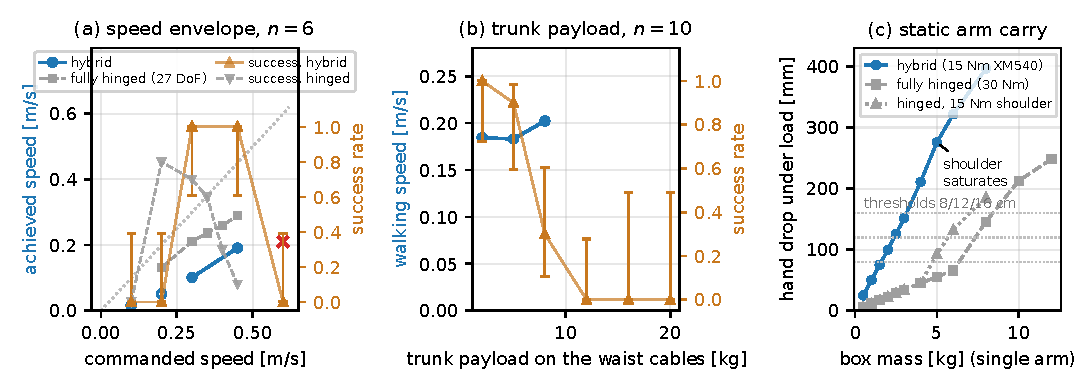
\includegraphics[width=0.98\textwidth]{sweeps.pdf}
\caption{Capability sweeps on the hybrid; error bars are Wilson 95\%
intervals on the success rate. (a) Achieved speed and success rate vs.\
commanded speed ($n=6$), with the fully hinged machine's envelope in grey:
the hybrid walks reliably in a 0.30--0.45\,m/s command band and tracks at
$\approx$42\%, against the hinged machine's 65\% tracking and 0.29\,m/s top
speed. Commands of 0.10--0.20\,m/s are not falls --- the robot stays upright
but undertracks below the walking threshold. (b) Trunk payload carried above
the tensegrity waist ($n=4$): reliable at 2\,kg, marginal to 8\,kg, and gone
by 12\,kg --- the cable torso mount is the binding constraint, where the
hinged machine's rigid trunk was flat to 20\,kg. (c) Static single-arm carry
with the 7-DoF arm: sag through the arm chain's compliance drops the load at
2.5\,kg with the XM540 shoulder at 71\% torque; the busiest waist cable
(orange, right axis) picks up the carry, a load path the hinged machine did
not have.}
\label{fig:sweeps}
\end{figure*}

\subsection{Capability envelope}
\label{sec:hybridenvelope}
Rerunning the fully hinged machine's capability sweeps on the hybrid
(Fig.~\ref{fig:sweeps}) quantifies what the two tensegrity joints and the
lighter arms cost and buy at the level of whole-machine capability.

\textbf{Speed.} The hybrid has a reliable command band rather than a smooth
degradation: \hsSpdThirtyRate{} at a commanded 0.30\,m/s
(\hsSpdThirtyV\,m/s achieved) and \hsSpdFortyFiveRate{} at 0.45
(\hsSpdFortyFiveV\,m/s), with every trial at 0.60 ending in a fall.
Below the band the machine does not fall --- at commands of 0.10--0.20\,m/s
it stays upright for the full 16\,s but covers too little ground to count,
walking at 0.02--0.05\,m/s. The gait reference's sway-and-step cycle has a
minimum viable tempo; below it the planner holds station. Tracking is the
larger difference: the hybrid achieves $\approx$42\% of its command where the
hinged machine achieved 65\%, because part of every push-off is stored in
the elastic network rather than delivered to the ground --- the same
compliance tax measured joint-by-joint in Sec.~\ref{sec:jointcount}.

\textbf{Trunk payload.} Boxes fixed to the torso ride \emph{above} the
tensegrity waist, so unlike on the hinged machine every added kilogram loads
the twelve waist cables. The envelope is correspondingly smaller:
\hsPayTwoRate{} at 2\,kg (\hsPayTwoV\,m/s, within noise of unloaded),
\hsPayFiveRate{} at 5, \hsPayEightRate{} at 8, and \hsPayTwelveRate{} from
12\,kg up --- against an envelope flat to 20\,kg on the rigid trunk. The
failures are informative: at 12\,kg and above every trial falls
\emph{backward} within the first strides, the loaded waist settling and
pitching the trunk aft faster than the planner's horizon can buy back. The
hinged machine's payload was tendon-limited at the leg; the hybrid's is
compliance-limited at the waist. A design that needs to carry more than
$\sim$8\,kg on the trunk should either stiffen the waist cage under load or
mount the payload below it, on the pelvis --- the co-design lever this sweep
isolates.

\textbf{Arm carry.} With the pelvis fixed (the E2 methodology) and the arm
PD-held in the forward carry pose, the 7-DoF arm holds \hsCarryMax\,kg
--- shoulder at \hsCarryUtil\% of its 15\,N\,m limit --- and drops the
2.5\,kg box, not by motor saturation but by \emph{sag}: at failure the
shoulder is at 71\%, and the accumulated deflection of seven
servo-compliant joints carries the hand past the drop threshold. The hinged
machine held 5\,kg with a 30\,N\,m shoulder. Halving the arm's drive class
(0.165\,kg XM540 vs.\ 0.96\,kg AK10-class) halves the carry, roughly
proportionally --- and the carry now has a load path the hinged machine
lacked: the busiest waist cable rises from 52\,N unloaded to
\hsCarryWaistT\,N under the held box, so arm payload on the hybrid is
bounded by waist cable rating as well as shoulder torque, a coupling an
outer design loop must price.

\subsection{What the hybrid says about the architecture question}
The hybrid resolves the split verdict of Sec.~\ref{sec:buys} into a working
design rule. The hinge-free joint contributes what it is measurably good at
--- impact attenuation at the contact end of the limb
(Sec.~\ref{sec:jointimpact}), wrench-closed compliance with an order of
magnitude cheaper actuation --- exactly where heel strike arrives. The hinges
contribute what they are good at: pose-independent torque at the joints that
size the gait. Neither pure architecture walks as well: the fully hinged
machine pays \bearingMass\,kg of bearings and forfeits impact tolerance
everywhere; the fully hinge-free machine of Sec.~\ref{sec:cellgraph} stands
but has no controller. The hybrid walks at \hybridSpeed\,m/s in \hybridRate{} of trials with the
full upper body, batteries and both tensegrity joints in place (0.29\,m/s
with the torso rigidly mounted), and every element of it is the choice the
measurements of this paper individually recommend.



\section{How Many Joints Does a Humanoid Need?}
\label{sec:jointcount}
The hybrid fixes one point on an axis that runs from a machine with no
bearings at all to one with a bearing at every degree of freedom. This
section walks that axis with variants of the \emph{same} robot --- identical
masses, drives, anthropometry and controller --- differing only in which
joints are bearings and which are cable interfaces, together with the two
endpoints built earlier in this work
(Table~\ref{tab:jointcount}).

\begin{table}[tb]
\centering
\caption{The joint-count axis. Middle rows are variants of the hybrid run
under its shipped controller configuration ($n=5$); the endpoints carry their
own best-known tuning. ``T-joints'' counts tensegrity (bearing-free) joints.}
\label{tab:jointcount}
\setlength{\tabcolsep}{2.6pt}\footnotesize%
\begin{tabular}{@{}lccccl@{}}
\toprule
variant & brgs & T-jts & walks & m/s & note\\
\midrule
pure tensegrity & 0 & all & --- & --- & stands only; no planner\\
\textbf{hybrid (design)} & 0.8\,kg & 3 & \textbf{\hybridRate} &
\hybridSpeed & impact $-$27..32\%\\
\;+ rigid waist & 0.8\,kg & 2 & \jcRWaistRate$^\dagger$ & --- &
tuning mismatch\\
\;+ rigid ankles & 0.8\,kg & 1 & \jcRAnkleRate & \jcRAnkleV & \\
\;+ both rigid & 0.8\,kg & 0 & \jcRBothRate & \jcRBothV & \\
fully hinged (27\,DoF) & 1.9\,kg & 0 & \walkRate$^\ddagger$ & \walkSpeed &
impacts $+$14..154\%\\
\bottomrule
\multicolumn{6}{@{}p{8.2cm}@{}}{\footnotesize $^\dagger$fails under the
hybrid's tuning; the same joint set walked 10/10 at 0.29\,m/s when tuned for
itself with simpler arms. $^\ddagger$own tuning; the fully hinged machine is
the source of the load traces and of experiments E1--E5.}
\end{tabular}
\end{table}

\subsection{Why any joints at all}
The pure-tensegrity endpoint answers this concretely, in three layers. First,
\emph{load path}: a hinge-free joint carries load only if the positive span
of its cable wrenches closes, which end-to-end cages do not provide ---
without the overlap-and-counter-winding geometry of
Sec.~\ref{sec:jointcell}, the machine is not even a structure. Second,
\emph{torque}: a bearing delivers its joint's full torque at every angle,
while a cable's moment arm is a function of pose; at the hip and knee, where
the gait demands 40--80\,N\,m through large excursions, the measured
authority of a cable joint collapses mid-stride
(Table~\ref{tab:authority}), and meeting it would take kilonewton tensions
on moment arms the cage cannot provide. Third --- and in practice first ---
\emph{planning}: every bearing removes three to five degrees of freedom from
the state a predictive controller must reason over. The hybrid's planner
handles 46 DoF at $0.3\times$ real time; the pure machine has 210, and no
controller in this work, or to our knowledge elsewhere, stabilises it. The
bearings at hips and knees are not a concession to tradition; they are what
makes the machine \emph{plannable} and its gait torques \emph{available at
every pose}.

\subsection{What removing joints buys}
Each bearing replaced by a cable interface buys, per the measurements in this
paper: \emph{impact attenuation} where it matters --- the cable ankle
attenuates drops by $27$--$32\%$ where a pin joint transmits them, and the
cable waist carries the torso at $\pm2^\circ$ through the gait; \emph{lighter
actuation} --- at a cable joint the moment arm is the cage radius, so
XM540-class drives (0.165\,kg) replace the AK10-class units (0.96\,kg) a
hinged ankle needs, an order of magnitude in actuation mass at that joint;
\emph{graceful degradation} --- no single cable of the twelve is structural,
where a bearing or its gearbox is a single point of failure; and
\emph{robustness to mass change} --- the compliant machine walked through an
asymmetric 2.5\,kg battery removal untouched. These are exactly the
properties E1--E3 showed the fully hinged machine forfeits.

\subsection{What removing joints costs}
The same rows quantify the price. \emph{Speed}: rigidising the tensegrity
joints raises gait speed monotonically ($\hybridSpeed \rightarrow
\jcRAnkleV \rightarrow \jcRBothV$\,m/s under one controller) --- compliance
taxes every stride, because part of each push-off goes into the elastic
network rather than the ground. \emph{Planner load}: every cable joint
returns six degrees of freedom to the state; the hybrid's two tensegrity
joints plus arm compliance took the planner from $0.6\times$ to $0.3\times$
real time, and live operation already requires slowing the simulation clock.
\emph{Tuning fragility}: the rigid-waist row is the sharpest lesson --- a
gait tuned for the compliant waist fails outright ($\jcRWaistRate$) when
that joint is rigidised, though the rigid configuration walks excellently
under its own tuning. Joint compliance is not a drop-in property; the whole
controller configuration co-varies with it, which is the co-design thesis of
this paper in miniature. \emph{Authority bookkeeping}: each cable joint must
be verified for wrench closure and pose-wide authority (Sec.~\ref{sec:authority});
a bearing needs neither.

\subsection{The design rule}
Between the endpoints the data support a simple allocation rule: \emph{put
bearings where the gait's torque lives, and cables where the world's impacts
arrive}. Hips and knees carry the largest, most pose-varied torques and no
impact --- bearings. Ankles meet the ground first and need an order of
magnitude less moment --- cables. The waist carries neither large torque nor
first impact; it is the marginal case, and the study shows it can go either
way: cable buys torso compliance at a speed and tuning cost, rigid buys
speed. Counting hardware, the hybrid's split saves 1.1\,kg of bearings over
the fully hinged machine while recovering the impact attenuation and
degradation tolerance that machine measurably lacks --- and unlike the pure
machine, it walks.

\section{What Tensegrity Buys}
\label{sec:buys}
The evidence separates into what the topology delivers as built, what it
delivers only hinge-free, and what it does not deliver at humanoid scale
regardless of topology.

\textbf{It buys mass, and mass is the point.} Every member is loaded along its
axis: cables cannot buckle and struts carry near-pure compression, where the
links of a conventional arm are cantilevers sized by bending. The consequence
is a change of regime rather than a marginal saving --- the compression
members are so far from buckling-critical that all \numStruts{} sit at minimum
manufacturable wall thickness, and the whole compression network is
\strutSpecMass\,kg on a 27.6\,kg machine. Table~\ref{tab:compare} puts that in
context: at fixed stature the mass spread across humanoids is nearly
threefold, and the two lightest are both tendon-driven with soft shells.

\textbf{It buys the transmission for free.} This is the property genuinely
specific to tensegrity rather than to tendon drive in general. In a
musculoskeletal humanoid the tendons act on a skeleton that must be built and
carried anyway; here the prestressed network that carries structural tension
\emph{is} the transmission, so proximal actuation costs no second mechanical
system. All \numMotors{} motors mount on belt, vest and proximal cuffs, and E4
shows the resulting distal-mass reduction is worth measurable gait robustness.

\textbf{It buys redundancy.} With \numActuatable{} actuatable cables of which
\numPassiveCables{} serve as passive prestress elements, no single cable is
structural: every single cut and every random loss of up to eight cables
survives standing plus a push, where one failed gearbox in a rigid robot is one
dead joint. The bound is that an adversary who knows the authority margins
topples the robot with eight.

\textbf{It buys impact tolerance --- but only without the hinge.} This is the
sharpest result in the paper. As built, the tension network makes impacts
worse, by \physOneLimpTen--\physOneLimpHundred\% at physical cable stiffness.
Built hinge-free, with cages overlapped by \jointOverlapMm\,mm so that the
cable interface achieves force closure, the same architecture attenuates peak
ground reaction by \jointImpactLo--\jointImpactHi\%
(Sec.~\ref{sec:jointimpact}). The property tensegrity is most often credited
with is real and is worth roughly a third of the landing force, and this design
forfeits it by using bearings. Recovering it costs a geometry change and
returns \bearingMass\,kg of bearings.

\textbf{It buys variable stiffness, as an actuation cost.} Antagonist
co-contraction modulates endpoint stiffness by $\stiffCoRatio\times$ with no
added hardware. What it does not buy is stiffness set at assembly: prestress
tunes stiffness only when the geometric term $T/L$ is comparable to the elastic
term $EA/L$, and with high-modulus rope it is \jointGeomElasticRope\% of it
(Sec.~\ref{sec:prestressscaling}). That conclusion is independent of the hinge
and independent of scale; it is a materials condition. Designers wanting
prestress-tunable stiffness must deliberately soften the tension members, which
trades against force bandwidth.

\textbf{It buys a manufacturing path.} The structure decomposes into short
discontinuous struts and sewn channels rather than machined shells, compatible
with cut-and-sew garment manufacture and with mounting in standard apparel ---
our longer-term aim, for which soft-exosuit work provides the load-path
precedents \cite{quinlivan2017exosuit}. This remains untested.

\textbf{What it does not buy.} Pose-independent torque. A rotary drive has the
same torque at every angle; a cable's moment arm is a function of
configuration, and that is the constraint that binds this design
(Sec.~\ref{sec:authority}). No topology removes it --- it can only be designed
against, which is what Sec.~\ref{sec:questions} argues should be the next
iteration's objective function.

\section{Open Research Questions}
\label{sec:questions}
The loop this paper runs is a design evaluator, not a design optimizer, and
what it has produced is a well-posed list of what to find out next.

\textbf{Can a hinge-free humanoid be planned for?} The structural half of this
question is now answered: overlapped cages give force closure and carry load
(Sec.~\ref{sec:jointcell}), and doing so recovers impact tolerance and
\bearingMass\,kg. The control half is open and is the harder one. A hinge-free
machine has six relative degrees of freedom per joint instead of one to three,
so the 27-DoF articulated abstraction that iLQG plans over disappears, and
with it the hierarchical decomposition this paper relies on. Whether a
predictive controller can stabilise a $\sim$90-DoF floating-strut humanoid, or
whether the right object is a reduced model that treats each cell as a
compliant joint with a tension-dependent stiffness, is the question that
decides whether this architecture is tensegrity or merely tensegrity-shaped.

\textbf{How should moment arms be designed?} Pose-dependent authority is the
binding constraint, and Eq.~\eqref{eq:authority} evaluated over the workspace
is a design constraint of the form $r_{\mathrm{eff}}(q)\ge\tau_{\max}/\Fmax$
for all reachable $q$ --- the wrench-feasible workspace condition
\cite{gouttefarde2007wfw} applied to a legged machine. Cage radius, drum radius
and lever geometry all move it at different mass costs. We have solved it by
inspection at four joints; solving it as a constrained optimization over cage
geometry is the natural next step and what the trade curves were built to feed.

\textbf{Which cables should be driven?} Selecting loop drives at the assembly
pose produced an actuation set that loses authority mid-stride. Loop selection
is combinatorial --- choose $m$ cable pairs from \numActuatable{} to maximize
worst-case authority over a trajectory distribution --- and it interacts with
the geometry question, since the best selection depends on the cage being
selected for.

\textbf{How soft should the tension members be?} Sec.~\ref{sec:prestressscaling}
turns a claimed advantage into a design variable. Series elasticity of
\kSeriesMin--\kSeriesMax\,kN/m is required merely to make prestress a practical
assembly operation; softer than that buys prestress-tunable stiffness and
impact attenuation, stiffer buys force bandwidth (Eq.~\ref{eq:bandwidth}) and
positional accuracy. That is a clean one-dimensional trade nobody in this
literature appears to have swept, and it is cheap to sweep with the tools here.

\textbf{Can tension-space planning be made real-time?} Direct MPC over
\numActuatable{} unilateral inputs sits at the edge of real time. The
hierarchical decomposition works but plans in a space the robot does not have,
which is how the authority shortfall went unnoticed for one design iteration.
A planner that respects unilaterality and pose-dependent moment arms natively
would close that gap --- and would be a prerequisite for the hinge-free machine
above.

\textbf{Does the mass advantage survive a full hardware accounting?} Rope is
\ropeMass\,kg; its terminations, nodes and bearings are
\termMass$+$\nodeMass$+$\bearingMass\,kg, and with bearings included the
structural budget does not close. Whether Table~\ref{tab:compare}'s advantage
survives wiring, sensing, channels and covers is unresolved and is what a build
would settle.

\textbf{And the standing caveats.} Everything here is simulated, with no tendon
friction, hysteresis, creep or cable mass, and with straight-line cable
routing. Cost of transport is \walkCot{}, five to fifteen times worse than
comparable machines; a light robot that is expensive to move undercuts the mass
argument, and where that energy goes --- tendon routing losses, the
saturated-torque gait, or the planner --- is unmeasured. The structural
mass-parity comparison against a rigid frame sized to the same loads (E9)
remains unrun.

\section{Conclusion}
A full-size humanoid can be laid out as a tensegrity, and predictive control is
a usable inner loop for designing one: prestress mathematics fixes the cell
geometry, tension-only mechanics fixes what the cables may do, the
wrench-feasibility bound decides controllability before any controller runs,
and iLQG given an analytic gait reference turns a statically sound structure
into a walking simulation whose load traces then size the actuators and
members. The first iteration produces a 1.65\,m, 27.6\,kg design --- the
lightest per unit height among size-matched humanoids --- that stands, recovers
from pushes, live-swaps its batteries, and walks 6\,m in a straight line at
\walkSpeed\,m/s in \walkRate{} of trials.

The measured case for tensegrity is that it buys mass, a transmission that
costs no second mechanical system, and redundancy. The case against the
\emph{implementation} is sharper and more useful: its joints are bearings, and
that single choice forfeits the impact tolerance the architecture can deliver.
A wrench-closure analysis shows the cables as routed could never have replaced
those bearings --- \wcThree{} of \wcTotal{} joints could be held by cable ---
and a hinge-free testbed shows what closes them: overlapping the cages by
\jointOverlapMm\,mm, which recovers \jointImpactLo--\jointImpactHi\% of impact
attenuation and returns \bearingMass\,kg of hardware. Prestress-tunable
stiffness is not recoverable by geometry at all; it is a condition on the ratio
of geometric to elastic stiffness, and high-modulus rope puts it out of reach.

The constraint that binds the walking design is neither mass nor strength but
pose-dependent torque authority: \authShortGaitBom{} of 27 degrees of freedom
fall short mid-stride under the specified actuation set, and re-planning inside
the achievable envelope localises the fault to the bill of materials rather
than the topology. Each of these findings names the parameter that would change
it --- \rNeedHip\,mm of effective moment arm against \rHaveHip\,mm today,
\jointOverlapMm\,mm of cage overlap against zero today, and a cable rating
$1.6\times$ the one specified. That is what we take the loop to be for.

\section*{Reproducibility}
The model generator, the MJPC task, all experiment scripts and the analysis
that produces every number in this paper are released with it. Each figure and
every quantity in the text is regenerated from logged runs by a single script,
so the text cannot drift from the data. The parametric generator emits the
joint-torque, cable-driven, hinge-free and physical-stiffness model variants
from one node graph, so every comparison in this paper can be reproduced from
a single command.

\bibliographystyle{IEEEtran}
\bibliography{../references/library}

\end{document}
